% Copyright (c) 2024, Francisco Fernandez
% License: CC BY-SA 4.0
%   https://github.com/fernandezfran/thesis/blob/main/LICENSE
\chapter{Modelo funcional de densidad de enlace fuerte}\label{ch:modelo}
\thispagestyle{empty}

\vspace{50pt}

\begin{adjustwidth}{50pt}{50pt}
    La capacidad de predicción de las simulaciones de dinámica molecular está 
    limitada principalmente por la escala temporal y por la fiabilidad del campo
    de fuerzas utilizado. La complejidad de las aleaciones amorfas de Li$_x$Si 
    requiere que ambas cuestiones se aborden simultáneamente. El método del 
    Funcional de Densidad de Enlace Fuerte (DFTB, \textit{Density functional 
    tight-binding}) aparece como una solución de complejidad intermedia a este
    problema, ya que es capaz de describir la naturaleza electrónica de diferentes 
    entornos, dándole una transferibilidad mayor que la de los campos de fuerzas clásicos, 
    a un costo computacional más bajo comparado a DFT (\textit{Density Functional
    Theory}). En este capítulo se presenta un conjunto de parámetros DFTB adecuados
    para modelar las aleaciones amorfas de Li$_x$Si. Dichos parámetros se 
    construyen haciendo especial hincapié en su transferibilidad para todo el 
    intervalo de carga. Esto se logra al introducir un algoritmo de optimización 
    que pesa las distintas estequiometrías para mejorar la predicción de algún 
    observable, en este caso sus energías de formación. El modelo resultante se 
    muestra robusto para la predicción de estructuras cristalinas y amorfas, 
    presentando una excelente concordancia con cálculos DFT y superando el 
    potencial ReaxFF del estado-del-arte para este sistema que se presentó en el
    capítulo anterior.
\end{adjustwidth}

\clearpage
\newpage
\thispagestyle{empty}
\mbox{}
\newpage

\section{Introducción}


\section{Métodos computacionales}

\subsection{Cálculos DFT}\label{s:dftcalc}

Los cálculos de DFT de las estructures cristalinas fueron obtenidos usando el 
paquete de simulación \path{GPAW} \cite{enkovaara2010, mortensen2005} del 
Entorno de Simulación Atómica \cite{larsen2017}. El paquete \path{GPAW} provee un 
algoritmo de grillado del espacio real basado en el método de la función de onda 
aumentada por proyector \cite{blochl1994} que utiliza la aproximación del núcleo 
congelado. Las coordenadas de Li, Li$_{15}$Si$_{4}$, Li$_{13}$Si$_{4}$, 
Li$_{7}$Si$_{3}$, Li$_{12}$Si$_{7}$, LiSi y Si se descargaron del Materials 
Project \cite{materials_project} (códigos mp: 135, 569849, 672287, 1201871, 1314, 
795 y 149) correspondiente al Li BCC, x $\approx$ 3.75, 3.25, 2.33, 1.71, 1 y
Si diamante, respectivamente. Los cálculos DFT se realizaron utilizando el 
funcional de intercambio-correlación PBE (Perdew-Burke-Ernzerhof) y la integración
de la zona de Brillouin se efectuó con grillas Monkhorst-Pack con una densidad
de 2.5 puntos $k$ por \AA$^{-1}$.

También se estudiaron, con cálculos DFT, estructuras amorfas de Li$_x$Si siguiendo
el protocolo de litiación propuesto por Chevrier y Dahn \cite{chevrier2009, 
chevrier2010}. Se utilizó un esquema de celda repetida con 12 átomos de silicio y 
$N$ de litio por celda unidad, con $N\in[0,45]$ cubriendo todo el intervalo 
$x\in[0,3.75]$. Cada estructura Li$_{N+1}$Si$_{12}$ se obtuvo agregando un átomo 
de litio en la esfera vacía más grande de la celda Li$_{N}$Si$_{12}$ y realizando
una optimización geométrica de las posiciones atómicas y del volumen de la celda.
En este caso, se realizaron los cálculos con el programa \path{QUANTUM} 
\path{ESPRESSO} \cite{quantum_espresso,quantum_espresso_advanced}, utilizando el 
funcional de intercambio-correlación PBE con una energía cinética de corte de 
1090 eV y una integración de la zona de Brillouin con grillas Monkhorst-Pack con 
una densidad de 7 puntos $k$ por \AA$^{-1}$. Las posiciones atómicas y el volumen 
de la celda se optimizaron utilizando el algoritmo BFGS hasta que la fuerza fuera 
menor a 0.08 eV/\AA\ para cada estructura.


\subsection{Detalles técnicos de DFTB}\label{ss:dftb}

El formalismo de DFTB ya fue introducido en el capítulo \ref{ch:metodos}, 
sección \ref{s:dftb}. A la hora de elegir el potencial de confinamiento de la
ecuación \ref{eq:dft} se mencionó que lo usual es elegir un parabólico, 
cuadrático, o una función de ley de potencias, siendo esta última opción la 
utilizada debido a que es la que está implementada en el código \path{Hotcent}
\cite{hotcent},
\begin{equation}\label{eq:vconf}
    V_{\text{conf}}(r)=\left(\frac{r}{r_0}\right)^{\sigma}
\end{equation}
donde $r_0$ y $\sigma$ son números reales que pueden ser elegidos de para cada 
orbital atómico $\phi$ y cada densidad $\rho^0$.

En la Tabla \ref{t:hubbard} se presentan las configuraciones electrónicas 
utilizadas, junto a las energías en el sitio de los orbitales de valencia y a 
los parámetros de Hubbard calculados, que se introducen en el segundo término
de la ecuación \ref{eq:dftb}.
\begin{table}[h!]
    \centering
    \caption{Configuraciones electrónicas, energías en el sitio de los orbitales
    de valencia y parámetros de Hubbard calculados con el funcional de intercambio
    y correlación PBE.}
    \setlength\extrarowheight{2pt}\stackon{%
    \begin{tabular}{l c c c c c}
        \toprule
        \textbf{Elemento} & 
        \textbf{Capa de valencia} &  
        \textbf{$\varepsilon_s$} &
        \textbf{$\varepsilon_p$} &  
        \textbf{$U_s$} & 
        \textbf{$U_p$} \\
        \midrule
        Li & 2s$^1$ & -0.105127 & -- & 0.167057 & -- \\
        Li & 3s$^2$3p$^2$ & -0.395452 & -0.150169 & 0.329247 & 0.244483 \\
        \bottomrule
    \end{tabular}
    }{}
    \label{t:hubbard}
\end{table}

El potencial de repulsión utilizado para definir la ecuación \ref{eq:rep} 
se ajustó utilizando el código \path{TANGO} \cite{tango}, donde el potencial 
repulsivo está dado por:
\begin{equation}\label{eq:v_rep}
    V_{\text{rep}}(r) = \begin{cases}
        e^{-a_1r+a_2}+a_3 & 0\le r<r_{\min}\\
        \displaystyle\sum_{i=2}^m c_i\left(r_{\text{cut}}-r\right)^i & r_{\min}\le r < r_{\text{cut}}\\
        0 & r_{\text{cut}} \le r
    \end{cases}
\end{equation}
los valores que se utilizan para $r_{\min}$ y $r_{\text{cut}}$ se encuentran
en la Tabla \ref{t:mincut}. Los parámetros $a_i$ se ajustan para reproducir las 
energías de DFT para cada estructura elegida para el entrenamiento utilizando el 
algoritmo de Levenber-Marquardt. Se eligió el grado del polinomio $m = 8$ y 
los coeficiente $c_i$ se optimizaron con un ajuste por cuadrados mínimos.

\begin{table}[h!]
    \centering
    \caption{Valores de $r_{\min}$ y $r_{\text{cut}}$ utilizados en la ecuación
    \ref{eq:v_rep}}
    \setlength\extrarowheight{2pt}\stackon{%
    \begin{tabular}{l c c}
        \toprule
        & 
        \textbf{$r_{\min}$ [\AA]} & 
        \textbf{$r_{\text{cut}}$ [\AA]} \\
        \midrule
        Si-Si & 1.7760 & 3.4410 \\
        Si-Li & 1.7925 & 4.1825 \\
        Li-Li & 1.9456 & 4.7360 \\
        \bottomrule
    \end{tabular}
    }{}
    \label{t:mincut}
\end{table}

Los códigos \path{Hotcent} y \path{TANGO} proveen valores por defecto para 
cualquier otro parámetro que no haya sido explícitamente descripto. 


\subsection{Algoritmo de ajuste}\label{s:algfit}

Para la obtención de los parámetros Li-Si de DFTB se siguió el 
método de aprendizaje descripto en los trabajos de van den Bossche \textit{et al.}
\cite{van2018, van2019}. Esto se realizó para dos conjuntos de parámetros, 
denotados como conjunto A y conjunto B, que difieren entre ellos en el ajuste
del término de la energía de bandas. En el conjunto A se ajusta la estructura 
de bandas de Li y Si por separado, mientras que en el conjunto B se utiliza para 
esto la estructura Li$_7$Si$_3$. La elección de esta última estructura se debe a
que el valor para la energía de formación es el menor entre todas las aleaciones
cristalinas consideradas \cite{materials_project}. La parametrización de los 
orbitales pseudoatómicos y de las densidades electrónicas consisten en optimizar 
los valores de $r_0$ y $\sigma$ en la ecuación \ref{eq:vconf} para ajustar la 
estructura de bandas de referencia de DFT. La Tabla \ref{t:vconf_params} muestra
los valores de los parámetros de confinamiento optimizados.
\begin{table}[h]
    \centering
    \caption{Parámetros del potencial de confinamiento $r_0$ y $\sigma$ para 
    los orbitales atómicos $\phi$ y las densidades $\rho^0$ de Li y Si}
    \setlength\extrarowheight{2pt}\stackon{%
    \begin{tabular}{l ccccc ccccc}
        \toprule
        &\multicolumn{5}{c}{\textbf{conjunto A}}&\multicolumn{5}{c}{\textbf{conjunto B}}\\
            \textbf{Elemento} & \textbf{$r_0(\phi)$} & \textbf{$\sigma(\phi)$} & \textbf{$r_0(\rho^0)$} & \textbf{$\sigma(\rho^0)$} & & & \textbf{$r_0(\phi)$} & \textbf{$\sigma(\phi)$} & \textbf{$r_0(\rho^0)$} & \textbf{$\sigma(\rho^0)$}\\
        \midrule
         Li & $4.899$ & $1.889$ & $7.233$ & $1.986$ & & & $4.843$ & $1.927$& $7.210$ & $1.999$\\
         Si & $4.558$ & $6.909$ & $6.318$ & $2.188$ & & & $3.556$ & $2.382$& $6.292$ & $1.891$\\
        \bottomrule
    \end{tabular}
    }{}
    \label{t:vconf_params}
\end{table}

Por otro lado, el conjunto de datos de entrenamiento requerido para ajustar el 
término de repulsión de pares se obtuvo utilizando las estructuras cristalinas 
ya mencionadas. Llámese $S$ al conjunto de estructuras cristalinas. A cada una de 
ellas se le realizaron compresiones y expansiones isotrópicas utilizando un 
factor de escaleo que varió de 0.4 a 1.45 con un equiespaciado de 0.05 unidades, 
generando así 22 estructuras por estequiometría. La energía de cada estructura se 
computó con DFT y se descartaron aquellas que superaban los 10 eV del mínimo de 
la estequiometría. De este procedimiento se obtuvieron 108 estructuras para el 
conjunto de entrenamiento. Para cada estructura $s$ de una dada estequiometría 
en $S$ ($s \in S$) se denota por $N_s$ la cantidad de estructuras asociadas a 
ella. Además, para cada estequiometría $s$, se denota con ${\bf r}^s_i$ la 
$i$-esima estructura y con $\check{{\bf r}}^s$ la estructura correspondiente a la
menor energía de DFT. Se usará el símbolo ``$\ \check{\ }\ $'' para denotar 
el argumento del mínimo de otras funciones.

Teniendo esto en cuenta, se obtiene el conjunto de parámetros 
$\check{\bf p} = \left( \left\{\check{c}_i\right\}, \left\{\check{a}_i\right\}\right)$ 
(ver ecuación \ref{eq:rep}) de DFTB que minimizan la sumatoria de los residuos 
de la energía
\begin{equation}\label{eq:e_res}
    \text{Res}_E({\bf p})=\sum_{s\in S}\sum_{i=1}^{N_s} \omega^s_i
    \left[E_{\text{DFT}}({\bf r}^s_i)-(E_{\text{DFTB}}({\bf r}^s_i;{\bf p})-C)\right]^2
\end{equation}
donde $C$ es una constante que desplaza la energía DFTB para corregir tendencias
sistemáticas a sobre- o sub-estimar energías \cite{van2018, van2019}, 
$E_{\text{DFTB}}({\bf r}^s_i;{\bf p})$ es la energía calculada utilizando DFTB con 
el conjunto de parámetros ${\bf p}$, $\omega_i^s$ permite controlar el peso 
relativo de cada estructura ${\bf r}^s_i$ en el proceso de ajuste.

Con el fin de minimizar la ecuación \ref{eq:e_res} es necesario elegir los pesos 
relativos $\omega_i^s$. En la referencia \cite{van2019}, los autores sugieren una 
distribución tipo Boltzmann
\begin{equation}\label{eq:omega}
    \tilde\omega^s_i=\exp\left(-\frac{E_\text{DFT}({\bf r}^s_i)-E_s}{b^s_i}\right)
\end{equation}
donde $b^s_i$ se considera proporcional al número de átomos $n^s_i$ en cada 
estructura y $E_s$ es la energía de referencia. Como se sugiere en la
documentación del código \path{TANGO} \cite{tango}, se puede fijar 
$b^s_i = 0.1 n^s_i$ eV y una elección adecuada para $E_s$ sería la energía más 
baja de la estequiometría $s$
\begin{equation}\label{eq:e_s}
  E_s=E_\text{DFT}(\check{{\bf r}}_s) \leq E_\text{DFT}({\bf r}^s_i) \quad \forall i \in [1,N_s].
\end{equation}
La motivación subyacente para esta ecuación es aumentar la precisión del modelo 
DFTB resultante para predecir estructuras de baja energía, renunciando a tener 
dicha precisión en estructuras de alta energía, que tienen menos probabilidad 
de ser encontradas durante una simulación canónica. Cabe destacar que este factor
de peso sólo se aplica a las estructuras de la estequiometría $s$ y no pesa las 
distintas estequiometrías.

Al elegir los pesos de las estructuras en el conjunto de entrenamiento en la 
ecuación \ref{eq:e_res}, se puede configurar el alcance de la aplicación para 
la parametrización de DFTB resultante. En otras palabras, para cada conjunto de 
pesos hay un conjunto de parámetros de DFTB ($\check{{\bf p}}$) distinto que 
minimiza la ecuación \ref{eq:e_res}. Basándose en esta idea, se puede elegir que 
los pesos sean
\begin{equation}\label{eq:omega2}
      \omega^s_i=\xi_s\tilde\omega^s_i=\xi_s\exp\left(-\frac{E_\text{DFT}({\bf r}^s_i)-E_s}{b^s_i}\right)
\end{equation} 
reteniendo así el enfoque en las estructuras de menor energía para cada 
estequiometría pero incluyendo un nuevo conjunto de coeficientes 
$\boldsymbol{\xi}$ $=\left(\xi_{\text{Li}},\cdots,\xi_{\text{Si}}\right)$ que 
permite controlar el peso relativo entre las distintas estequiometrías. Con esta 
definición, los parámetros óptimos de DFTB para la ecuación \ref{eq:e_res},
$\check{{\bf p}}$, pueden considerarse como una función que depende de 
$\boldsymbol{\xi}$, $\check{{\bf p}}(\boldsymbol{\xi})$. Lo cual 
introduce un segundo proceso de optimización para obtener los coeficientes 
$\check{\boldsymbol{\xi}}$.

El objetivo final de este capítulo es la parametrización de un modelo DFTB que 
permita luego simular la litiación de ánodos de silicio. Este es un proceso muy 
complejo ya que involucra distintos entornos químicos, con un intervalo amplio de
composiciones de Li$_x$Si. Sin embargo, es importante que la parametrización
mantenga su precisión para el mayor rango posible de concentraciones, para evitar 
la necesidad de cambiar de modelo \say{\textit{on-the-fly}} durante una simulación,
por lo que se requiere que la parametrización sea lo más transferible posible 
entre las distintas estequiometrías. En este sentido, el objetivo principal de la 
parametrización es que la misma realice predicciones fiables de algún observable, 
en este caso de las energías de formación relativas por átomo (definidas en la 
ecuación \ref{eq:formacion}) evaluadas en las estructuras 
$\lbrace \check{\mathbf{r}}_s \rbrace$. Por lo tanto, se 
optimizan los valores de los coeficientes $\check{\boldsymbol{\xi}}$ tal que 
minimizan la sumatoria de los residuos de las energías de formación relativas por 
átomo
\begin{equation}\label{eq:fres}
    \text{Res}_F(\boldsymbol{\xi}) = \sum_{s\in S} \left[F_\text{DFT}(\check{{\bf r}}^s)-F_\text{DFTB}(\check{{\bf r}}^s;\check{{\bf p}}({\boldsymbol{\xi}}))\right]^2
\end{equation}
La minimización de este residuo resulta en un conjunto de parámetros de DFTB
$\check{{\bf p}}(\check{\boldsymbol{\xi}})$ óptimo en el conjunto de 
entrenamiento donde las estequiometrías también son pesadas para dar un residuo
mínimo en su energía de formación.

En la Figura \ref{fig:diagrama} se muestra un diagrama de flujo con los pasos 
principales del algoritmo de ajuste descripto arriba. La minimización de la 
ecuación \ref{eq:e_res} se realiza con el código \path{TANGO} \cite{tango}. Para
minimizar la ecuación \ref{eq:fres}, se desarrolló un programa llamado 
\path{Milonga} que ejecuta varias instancias de \path{TANGO}, una por cada
evaluación de Res$_F(\boldsymbol{\xi})$ requerida por el proceso de minimización.

\begin{figure}[h!]
    \centering
    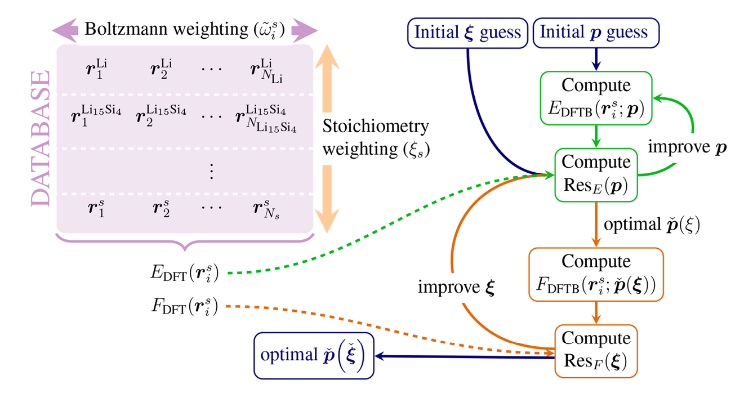
\includegraphics[width=\textwidth]{Silicio/modelo/metodos/diagrama.png}
    \caption{Diagrama de flujo del algoritmo de ajuste. Se realizan dos
    procedimientos de optimización anidados: la minimización de Res$_E$ (ecuación 
    \ref{eq:e_res}) utilizando el código \texttt{TANGO} \cite{tango} (resaltado en
    verde) y la minimización de Res$_F$ (ecuación \ref{eq:fres}) utilizando un 
    código llamado \texttt{Milonga} (resaltado en naranja). Cada mejora de los pesos
    $\boldsymbol{\xi}$ requiere una minimización completa de Res$_E$ para obtener 
    los parámetros óptimos DFTB asociados $\check{{\bf p}}(\boldsymbol{\xi})$.}
    \label{fig:diagrama}
\end{figure}


\section{Resultados}

\section{Introducción}


\subsection{Comportamiento electroquímico}

\subsubsection{Cambio de volumen fraccionario}

El cambio de volumen fraccionario puede definirse utilizando una normalización 
relativa al número de átomos de Si en la estructura de acuerdo a
\begin{equation}\label{eq:fvc}
    \text{fvc} = \frac{N_{\text{Si}}}{V_{\text{Si}}} \left( \frac{V_{\text{Si},x}}{N_{\text{Si},x}} - \frac{V_{\text{Si}}}{N_{\text{Si}}} \right),
\end{equation}
donde $V_{\text{Si}}$ y $N_{\text{Si}}$ son el volumen y el número de átomos de 
Si en la celda unidad de c-Si, $V_{\text{Si},x}$ y $N_{\text{Si},x}$ son el 
volumen y el número de átomos de Si
en la celda de simulación para el valor correspondiente de $x$. En la Figura
\ref{fig:fvc} se muestran los valores calculados a partir de la ecuación 
\ref{eq:fvc} para las distintas estructuras de Li$_x$Si estudiadas. En la misma 
se comparan los valores obtenidos con datos experimentales de AFM (\textit{atomic 
force microscopy}, sus siglas en inglés) medidos por Beaulieu \textit{et al.} 
~\cite{beaulieu2003} y con predicciones de DFT con un cambio volumétrico fijo 
utilizado por Chevrier y Dahn ~\cite{chevrier2009}. Los mismos muestran que el
potencial ReaxFF proporciona una tendencia correcta, tanto cualitativa como 
cuantitativamente.
\begin{figure}[th]
    \centering
    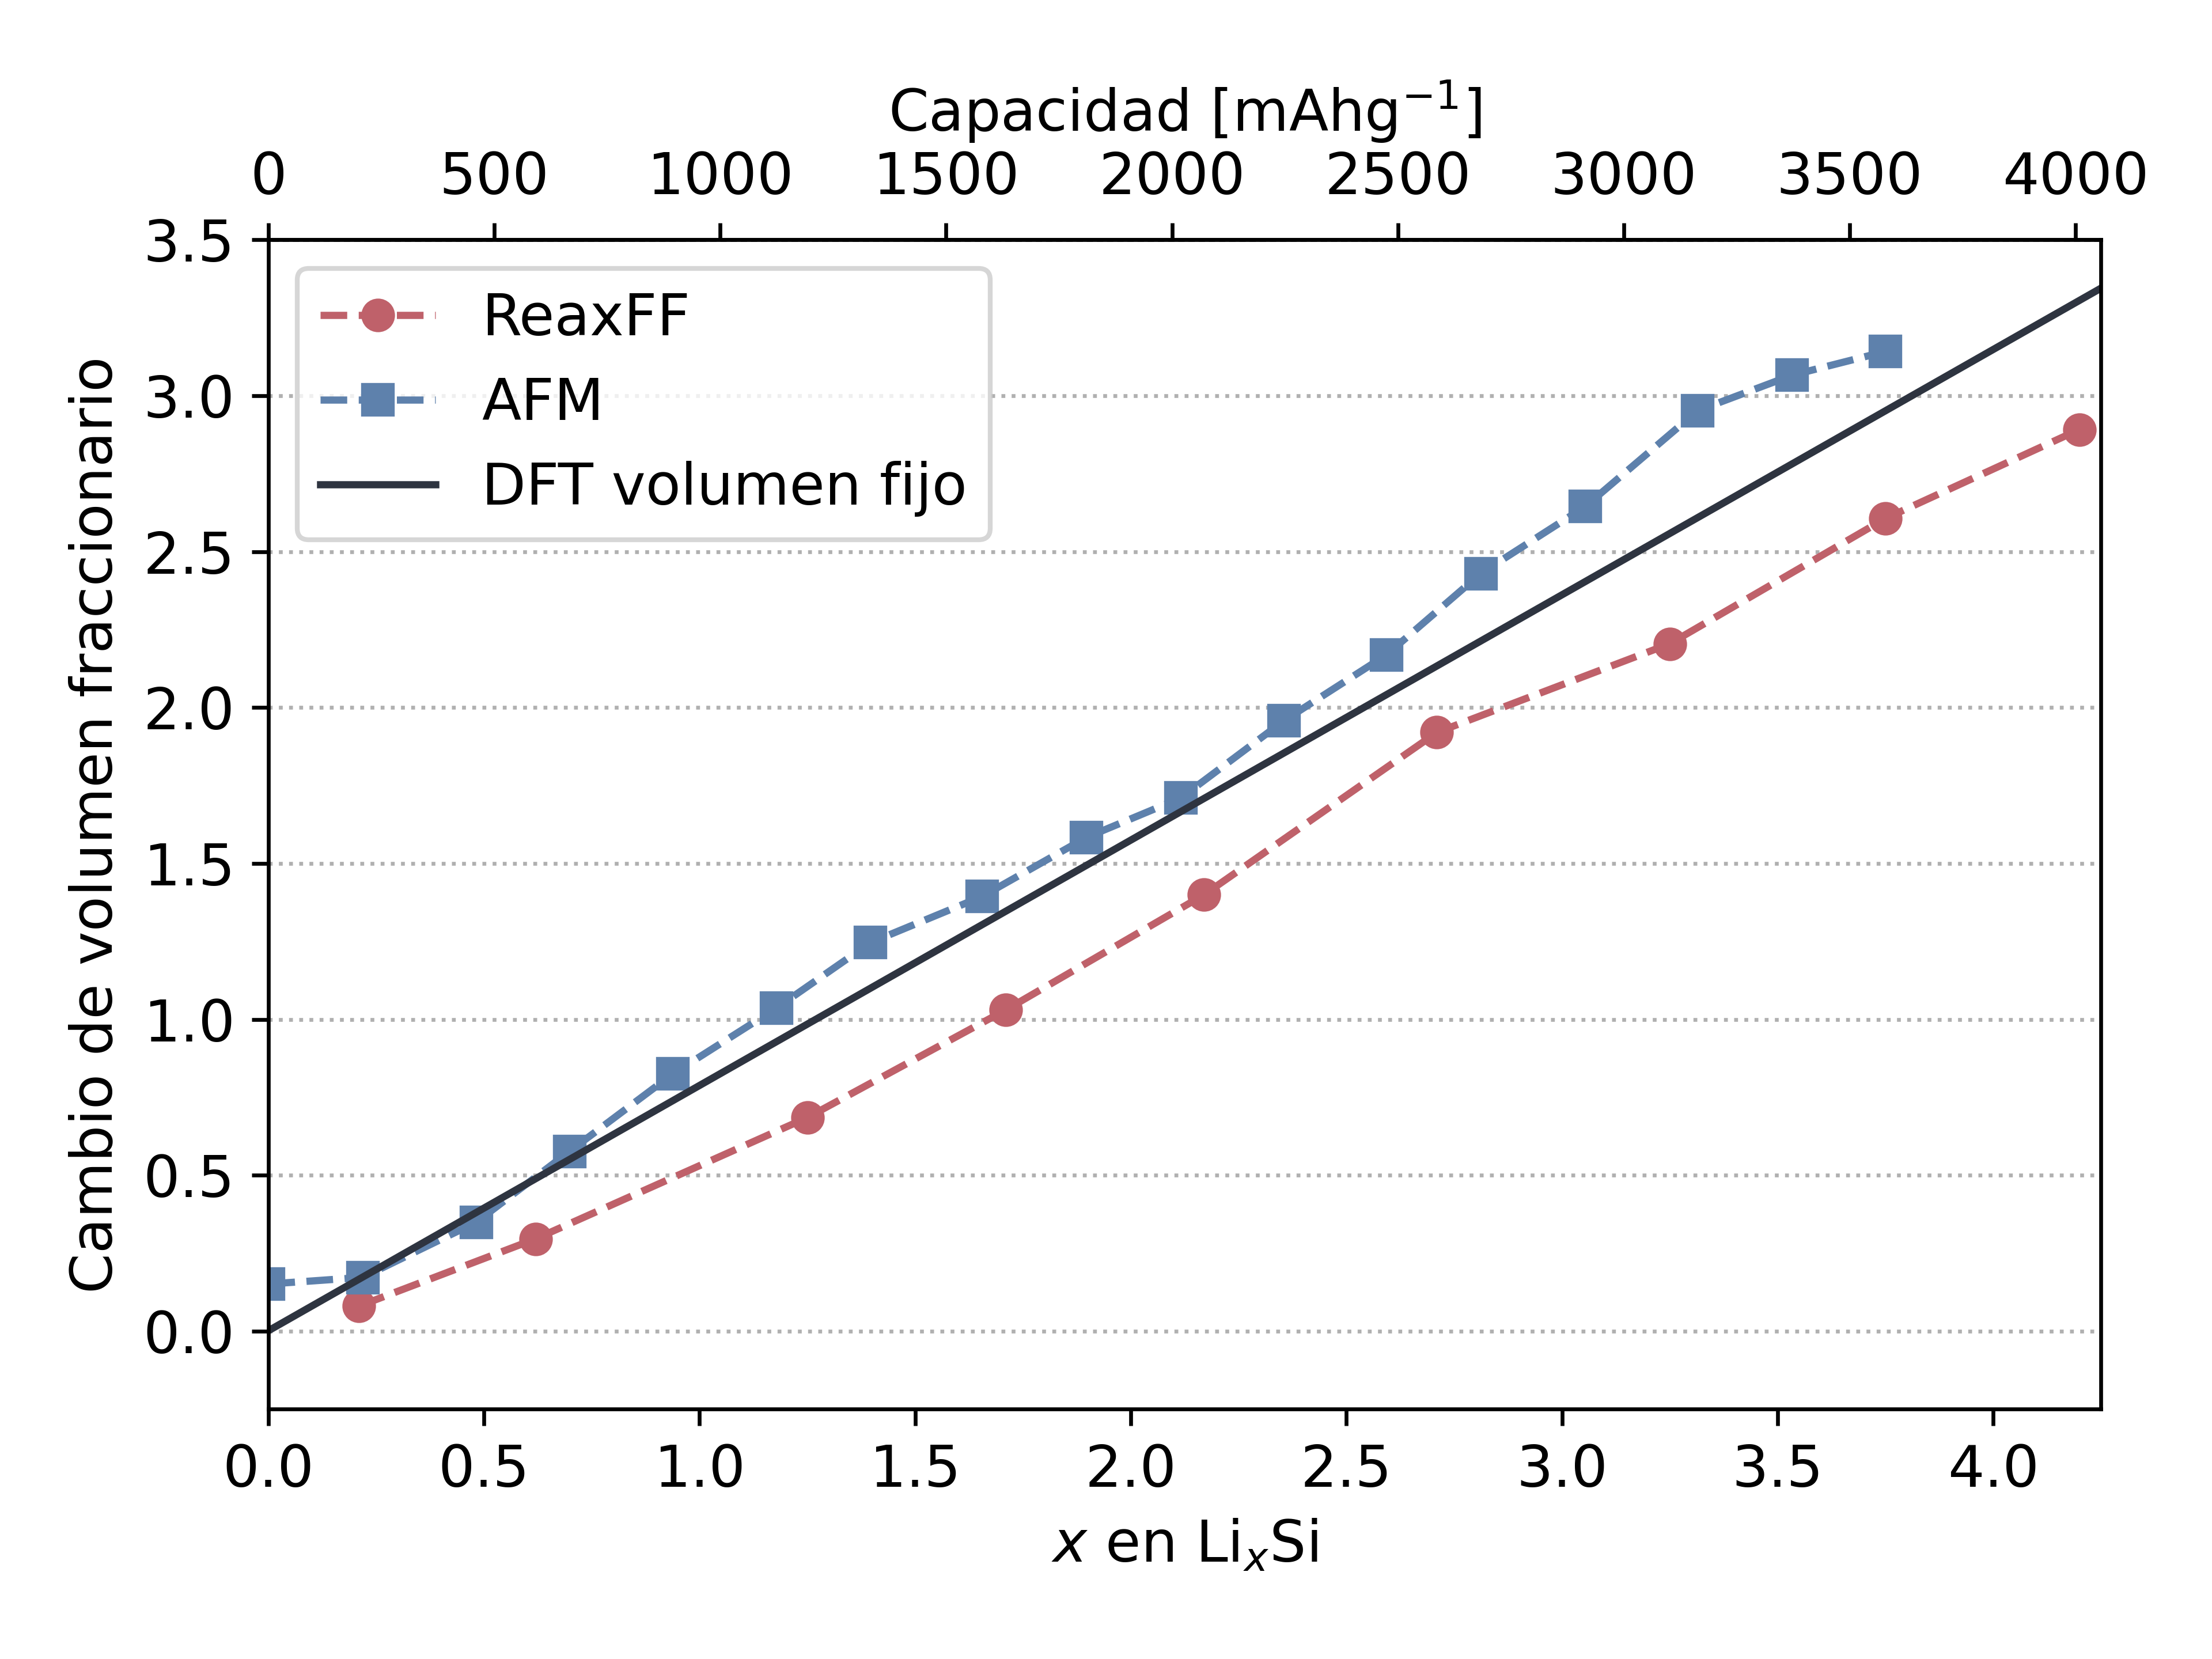
\includegraphics[width=0.8\textwidth]{Silicio/caracterizacion/resultados/electroquimica/fvc.png}
    \caption{Cambio de volumen fraccionario en función de la composición de la 
    aleación. Los valores experimentales de AFM se muestran con cuadrados azules, 
    la línea recta se corresponde con cálculos de DFT y los círculos rojos son 
    resultados de este trabajo.}
    \label{fig:fvc}
\end{figure}

\subsubsection{Voltaje}

\begin{table}[h]
    \centering
    \caption{Energías de formación obtenidas a través de la ecuación \ref{eq:fe}}
    \setlength\extrarowheight{2pt}\stackon{%
    \begin{tabular}{c c}
        \toprule
        \textbf{x en Li$_x$Si} & 
        \textbf{Energía de formación [eV]} \\ 
        \midrule
        0.21  &  0.503 $\pm$ 0.003 \\
        0.62  &  0.121 $\pm$ 0.007 \\
        1.25  & -0.12 $\pm$ 0.01 \\
        1.71  & -0.236 $\pm$ 0.007 \\
        2.17  & -0.355 $\pm$ 0.008 \\
        2.71  & -0.410 $\pm$ 0.007 \\
        3.25  & -0.52 $\pm$ 0.01 \\
        3.75  & -0.62 $\pm$ 0.01 \\
        4.20  & -0.699 $\pm$ 0.008 \\
        \bottomrule
    \end{tabular}
    }{}
    \label{t:fe}
\end{table}
Las energías obtenidas pueden ser utilizadas para evaluar el funcionamiento del 
modelo para predecir propiedades electroquímicas, como fue sugerido por Chevrier
y Dahn ~\cite{chevrier2009}. Primero, se define la energía de formación de las 
distintas estructuras amorfas como
\begin{equation}\label{eq:fe}
    E_f(x) = E_{\text{Li}_x\text{Si}} - (x E_{\text{Li}} + E_{\text{Si}}),
\end{equation}
donde $E_{\text{Li}_x\text{Si}}$ es la energía de la aleación Li$_x$Si por átomo 
de Si, $E_{\text{Li}}$ y $E_{\text{Si}}$ son las energías cohesivas de Li y Si
en sus fases cristalinas. Usando
la ecuación \ref{eq:fe} como aproximación a la energía de formación de Gibbs, el 
potencial \textit{versus} Li metálico de Li$_x$Si puede obtenerse a partir de
\begin{equation}\label{eq:voltaje}
    V(x) = - \frac{dE_f(x)}{dx},
\end{equation}
donde $V$ es el potencial. Los datos obtenidos así pueden compararse con valores
experimentales y computacionales previos. Las energías de formación calculadas
a partir de la ecuación \ref{eq:fe} se muestran en la Tabla \ref{t:fe}. 
Si se realiza un \textit{spline} a estos valores, mostrados en el recuadro de la
Figura \ref{fig:voltaje}, se obtienen los valores de $V(x)$ a partir de la ecuación
\ref{eq:voltaje}, que se grafican en función de la composición en la Figura 
\ref{fig:voltaje} con una línea roja. Para comparar, se incluye en la misma Figura
las curvas experimentales medidas para la litiación y la delitiación de silicio
amorfo ~\cite{hatchard2004} y la curva teórica de cálculos de primeros principios 
~\cite{chevrier2009}. Se puede afirmar que los resultados obtenidos con el ReaxFF 
son satisfactorios.
\begin{figure}[th]
    \centering
    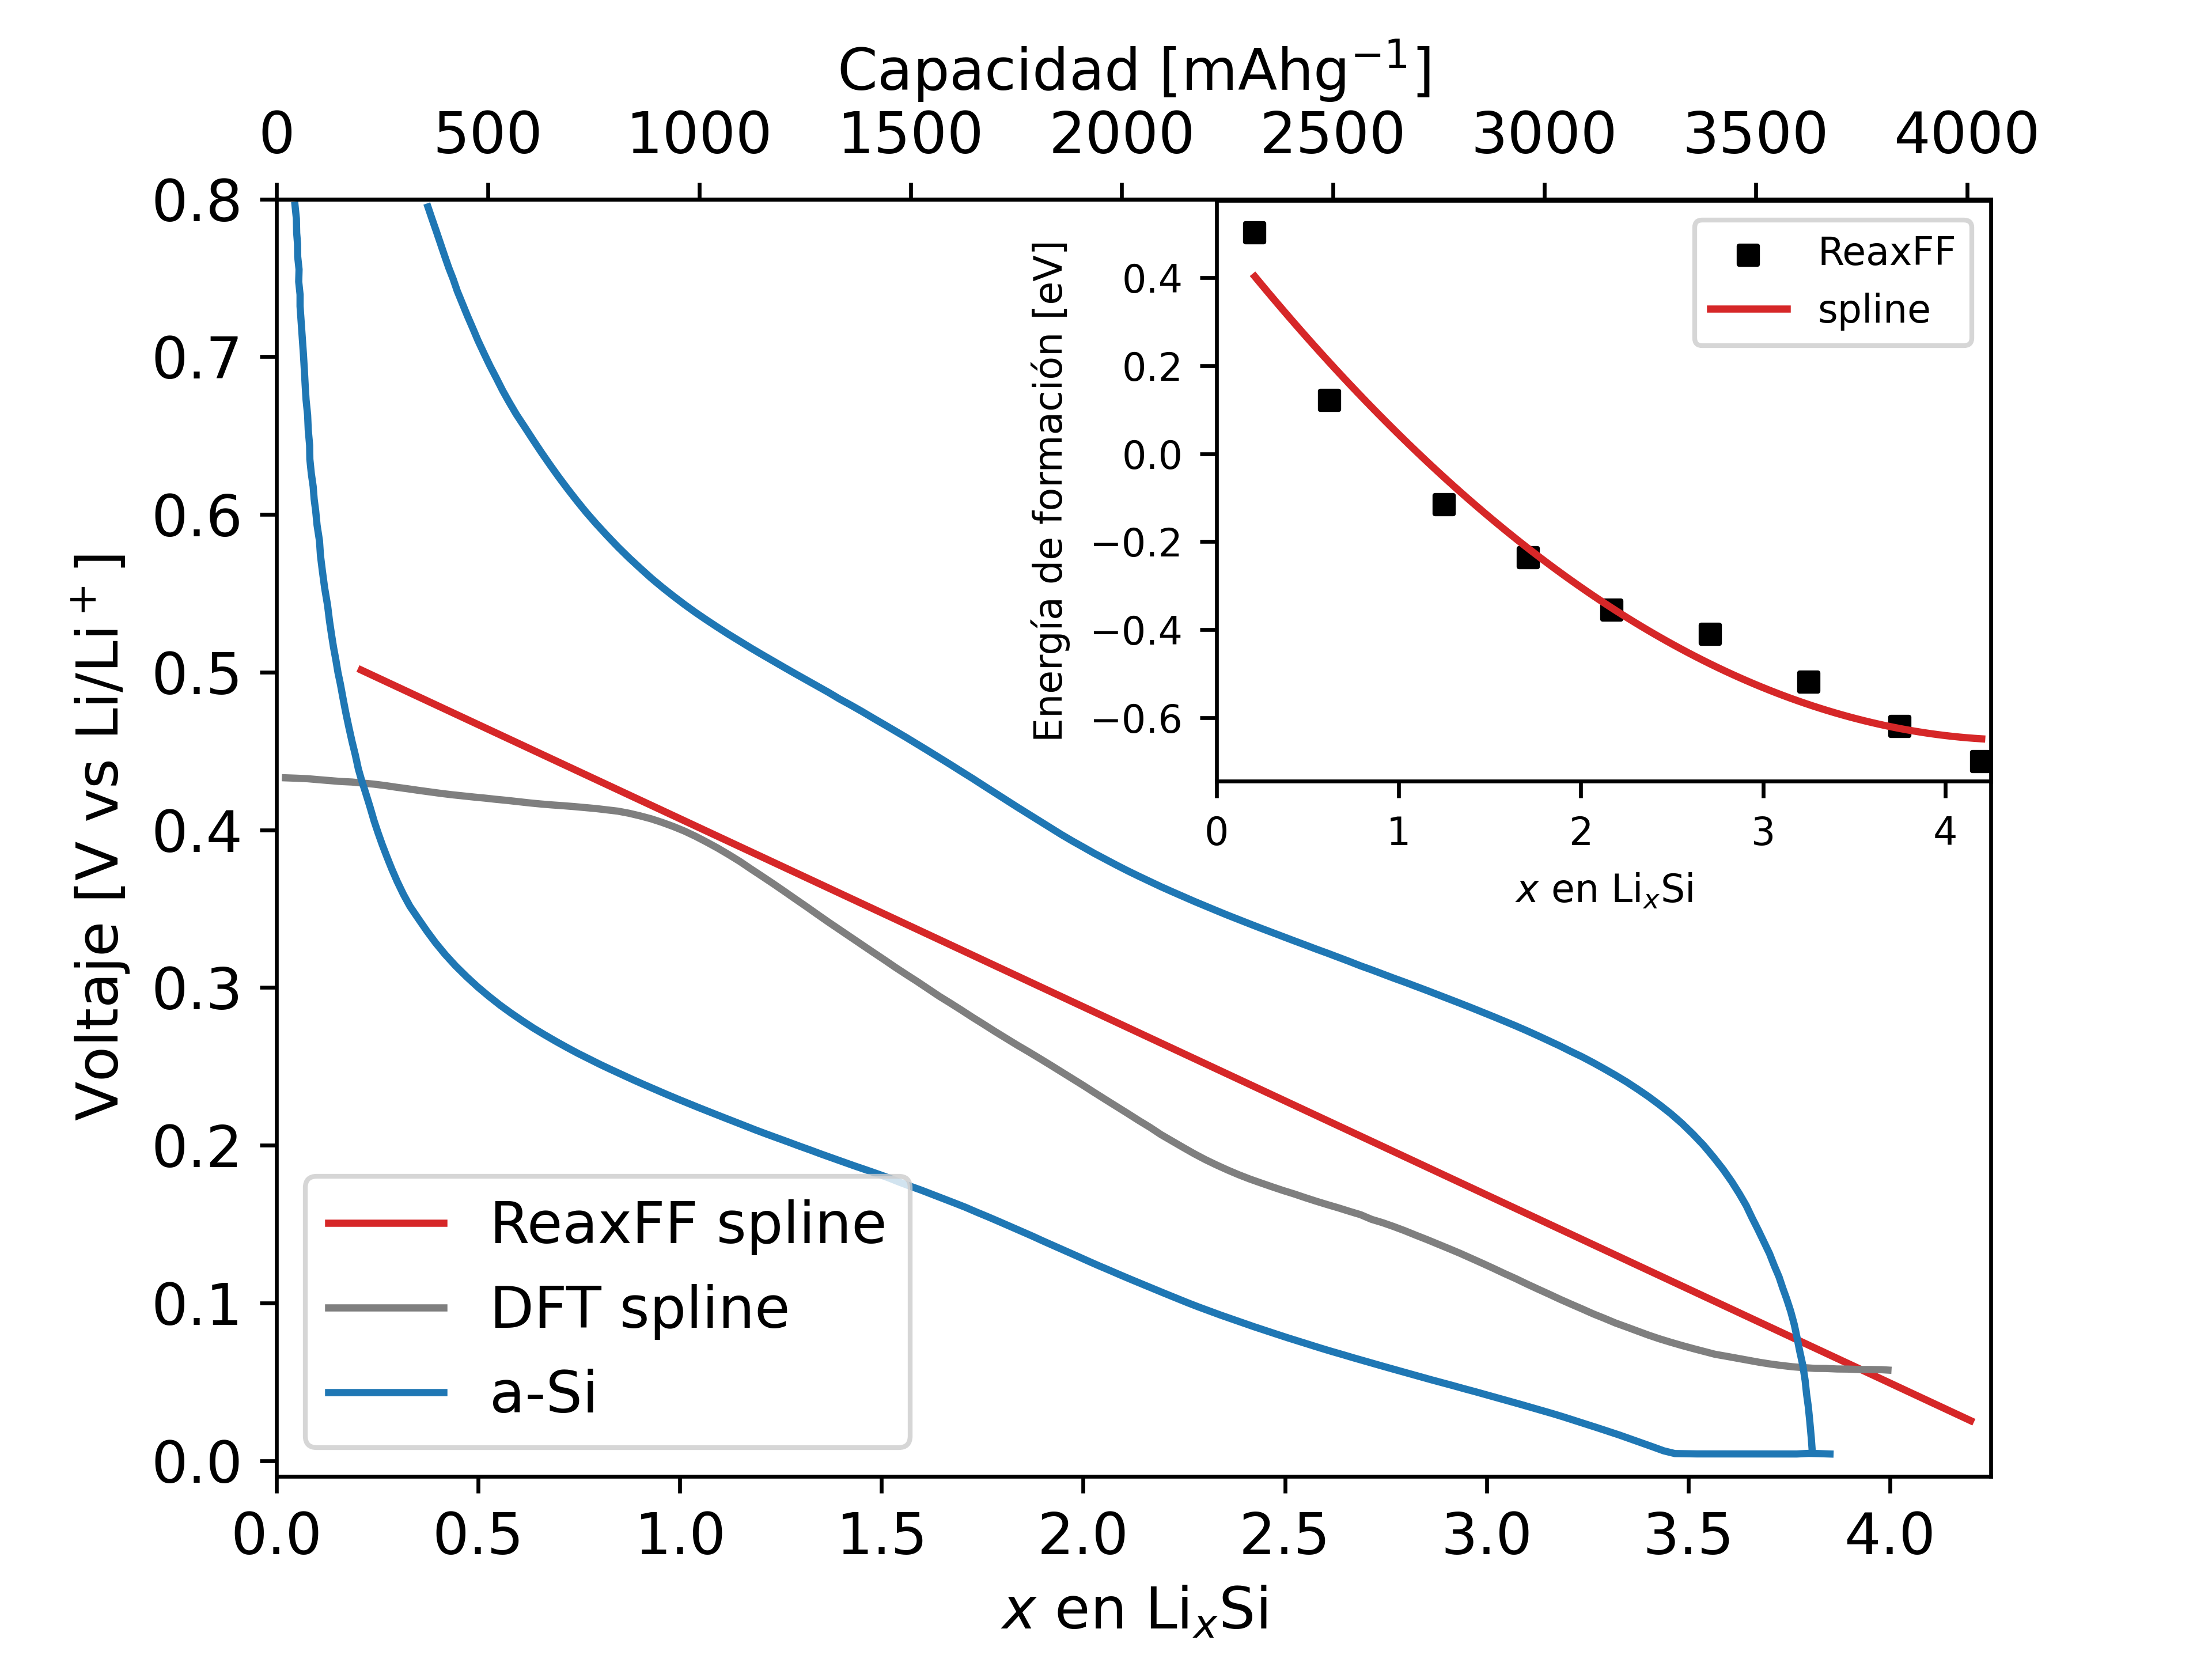
\includegraphics[width=0.8\textwidth]{Silicio/caracterizacion/resultados/electroquimica/voltaje.png}
    \caption{Curvas potencial-concentración para la litiación de ánodos de Si.
    La línea negra corresponde a cálculos de DFT, las líneas azules a 
    curvas medidas experimentalmente en la litiación de Si amorfo y la línea 
    roja es la derivada del \textit{spline} ajustado a los datos de la energía 
    de formación obtenidos con el ReaxFF, presentados en el recuadro.}
    \label{fig:voltaje}
\end{figure}


\subsection{Amorfización del silicio mediante un templado simulado y análisis de la función de distribución radial (RDF)}\label{s:rdfb}

Por último, las mayores discrepancias entre las energías de formación calculadas con DFTB
con respecto a DFT se corresponden a estructuras de silicio amorfo, por lo cual,
se realizó una evaluación extra para este caso. En la Figura \ref{fig:rdfb} se 
muestran las RDFs Si-Si (ver ecuación \ref{eq:rdf}) obtenidas por un templado simulado para cada una de las
parametrizaciones. Además, se compara con el potencial previo de ReaxFF 
\cite{fan2013} y con una determinación experimental \cite{laaziri1999}. Para 
obtener las estructuras amorfas se comenzó con una celda de c-Si con 64 átomos 
a la cual se le realizó un templado simulado en el ensamble $NVT$ utilizando el 
termostato de Nosé-Hoover. El mismo consistió en una etapa inicial de 
calentamiento lineal desde temperatura ambiente hasta 3000 K durante 100 ps, luego una
termalización a dicha temperatura por 600 ps y, por último, un enfriamiento 
exponencial de 600 ps hasta llegar a temperatura ambiente. Para todas las etapas
se utilizó un paso temporal de 1 fs. Para el cómputo de las RDFs que se muestran
en la Figura \ref{fig:rdfb} se equilibró la estructura alcanzada a temperatura 
ambiente durante 100 ps. Puede destacarse que los resultados del conjunto B de parámetros muestran
una concordancia excelente con los datos experimentales de la referencia 
\cite{laaziri1999}, lo que convierte a esta parametrización en la más adecuada
para simulaciones futuras. Los archivos de dichos parámetros están disponibles
en un repositorio público \cite{dftb_lisi}.
\begin{figure}[h!]
    \centering
    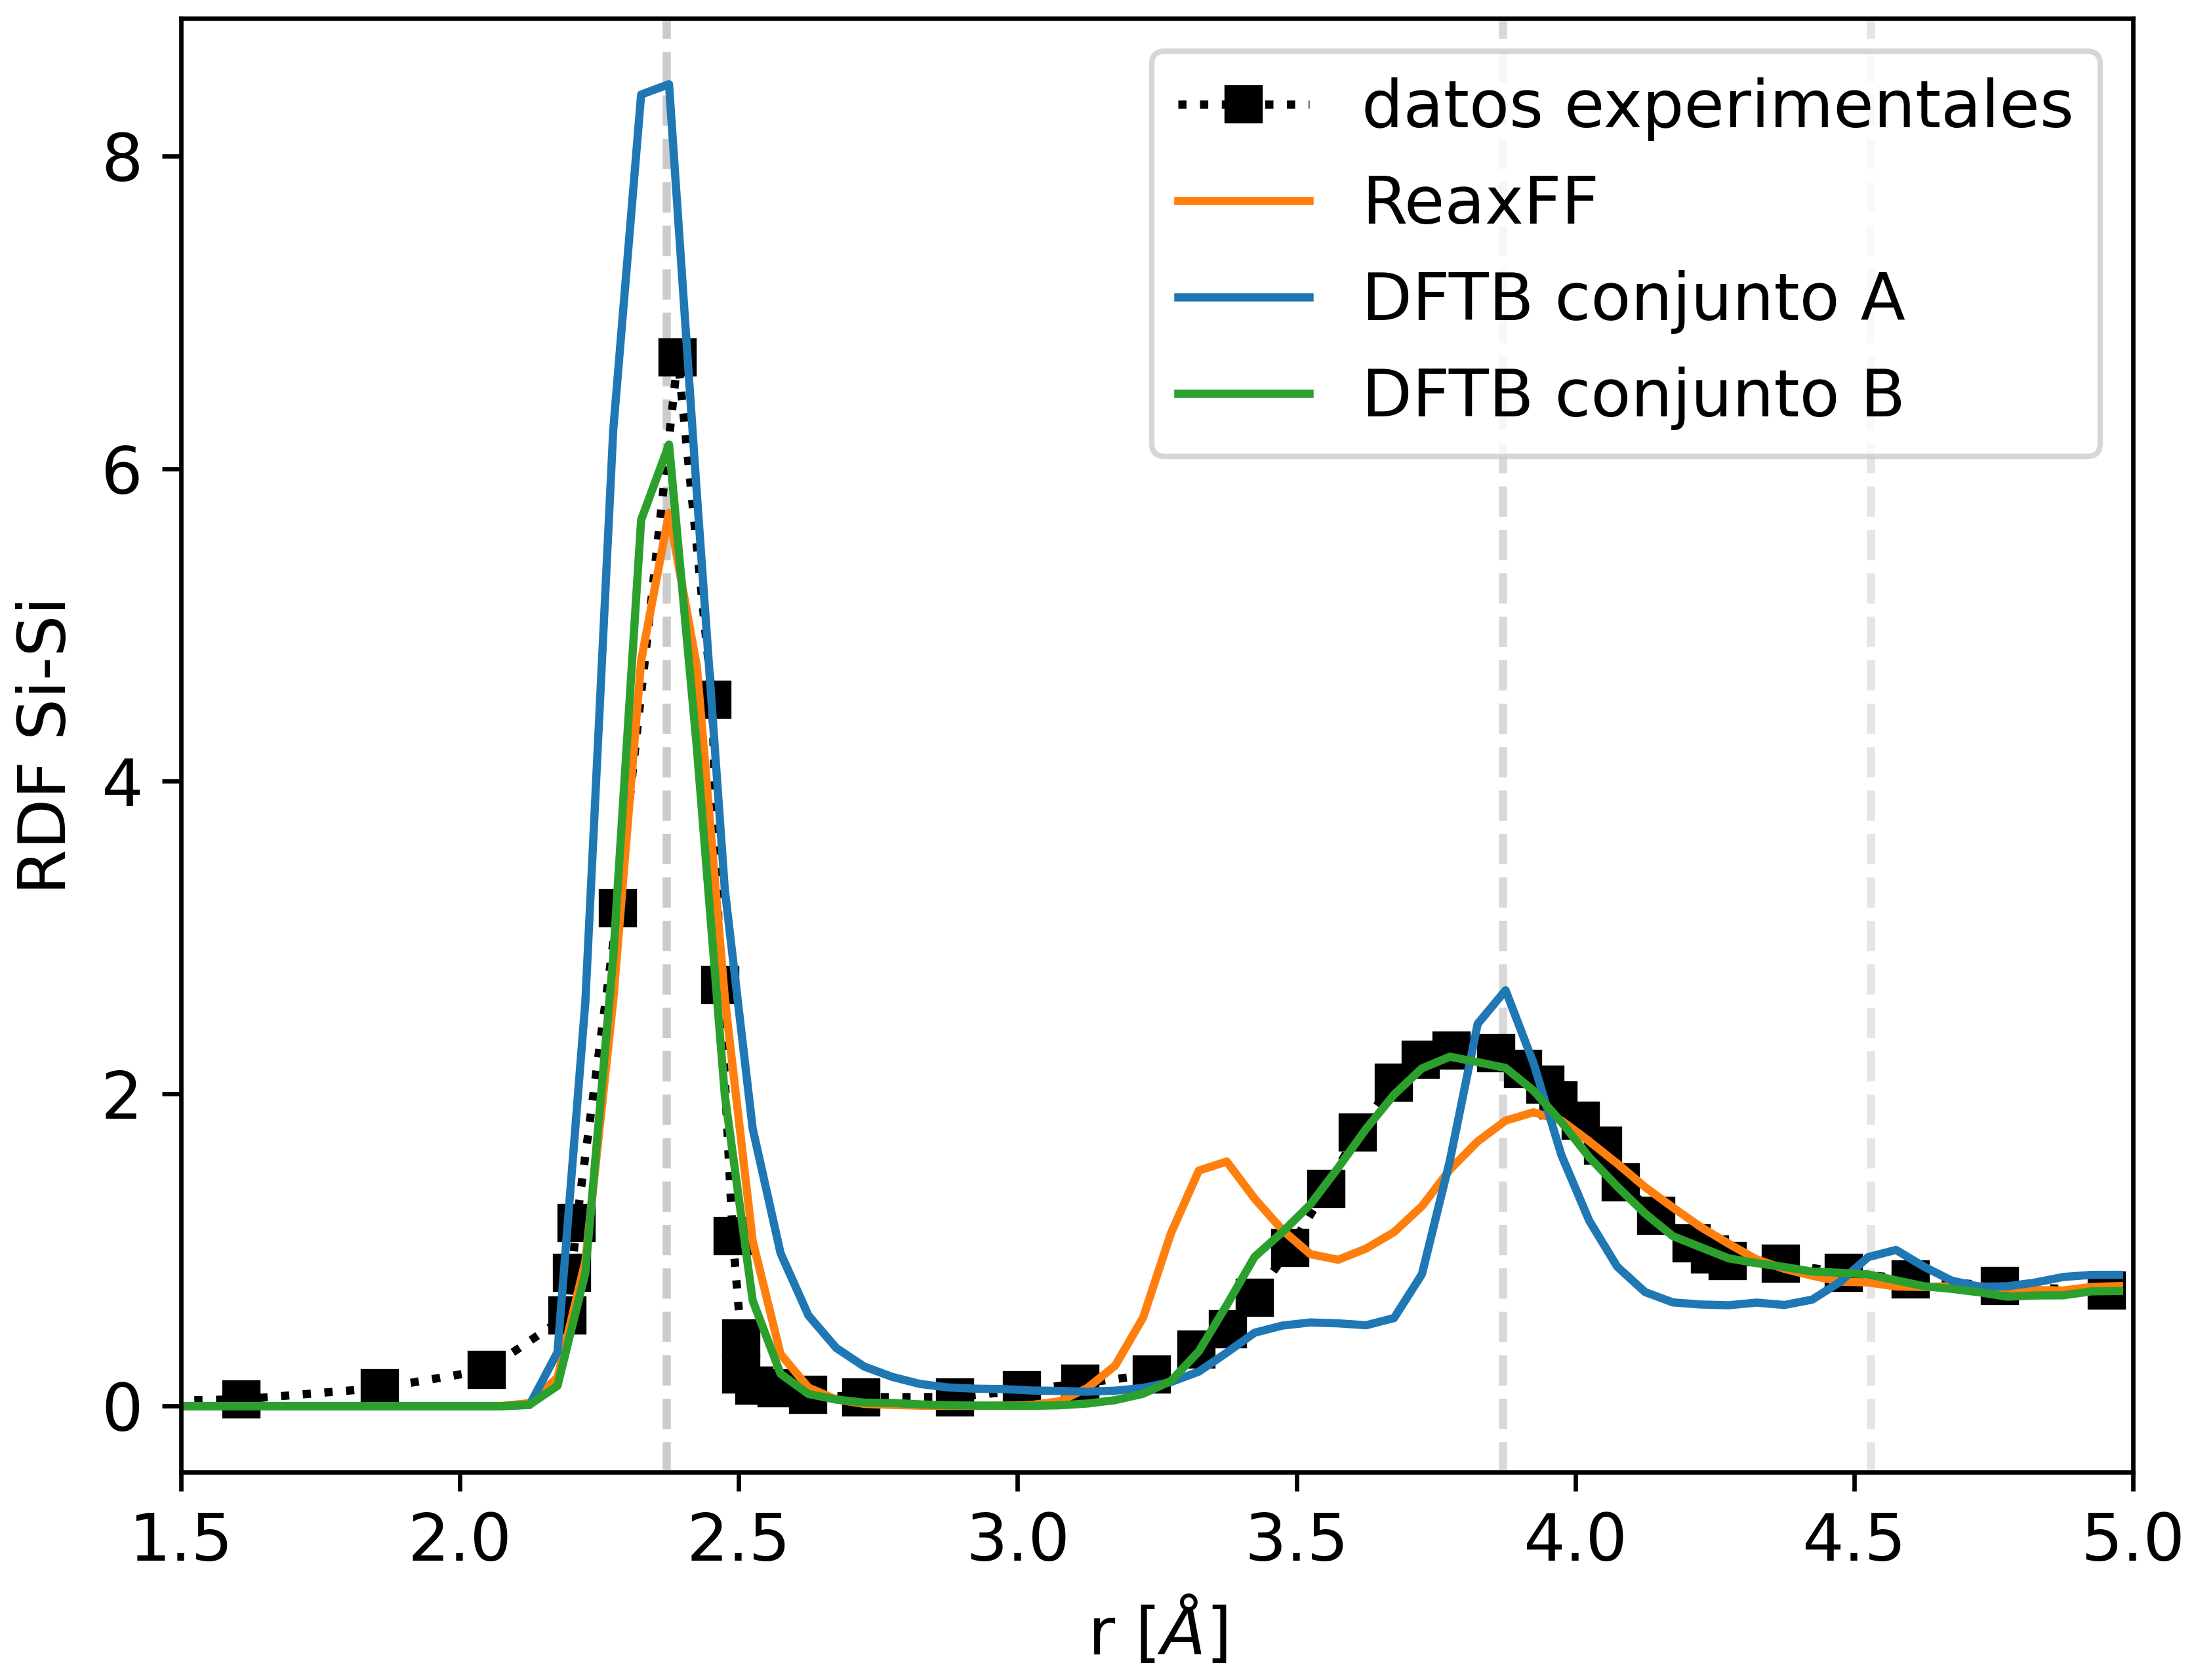
\includegraphics[width=.7\textwidth]{Silicio/modelo/resultados/rdf/rdf.png}
    \caption{Función de distribución radial (RDF) de silicio amorfo para los
    conjuntos A y B de parametrizaciones. Los resultados se comparan con 
    mediciones de la referencia \cite{laaziri1999} y con los resultados obtenidos
    utilizando el ReaxFF \cite{fan2013}. Las líneas grises discontinuas verticales
    muestran dónde estarían los picos del silicio cristalino a 0 K. Se encuentra 
    una concordancia excelente entre el experimento y la parametrización del 
    conjunto B.}
    \label{fig:rdfb}
\end{figure}


% Copyright (c) 2024, Francisco Fernandez
% License: CC BY-SA 4.0
%   https://github.com/fernandezfran/thesis/blob/main/LICENSE
\subsection{Número de coordinación}

De la misma manera que se utilizaron las distribuciones radiales parciales, se pueden
obtener los números de coordinación para un dado tipo de átomo utilizando la ecuación
\ref{eq:cn} definida en la sección \ref{ss:cn} con la $g(r)$ correspondiente. Debido
a que en los materiales amorfos la primera y la segunda esfera de coordinación pueden 
llegar a estar superpuestas, el límite superior de integración no está definido 
unívocamente para todas las concentraciones consideradas \cite{lamparter1995}.
El número de coordinación promedio para átomos de Si vecinos de otros átomos 
de Si se calculó utilizando un radio de 
corte de 3 \AA. Lo mismo se realizó para Li-Li definiendo un radio de corte de 
4 \AA. Para el caso de Si-Li se utilizó el criterio de considerar como radio de 
corte el valor $r$ para el cual la $g(r)$ presenta un mínimo entre los dos picos
a primeros y segundo vecinos. Los resultados se muestran en la Figura 
\ref{fig:cn}a.
\begin{figure}[h!]
    \centering
    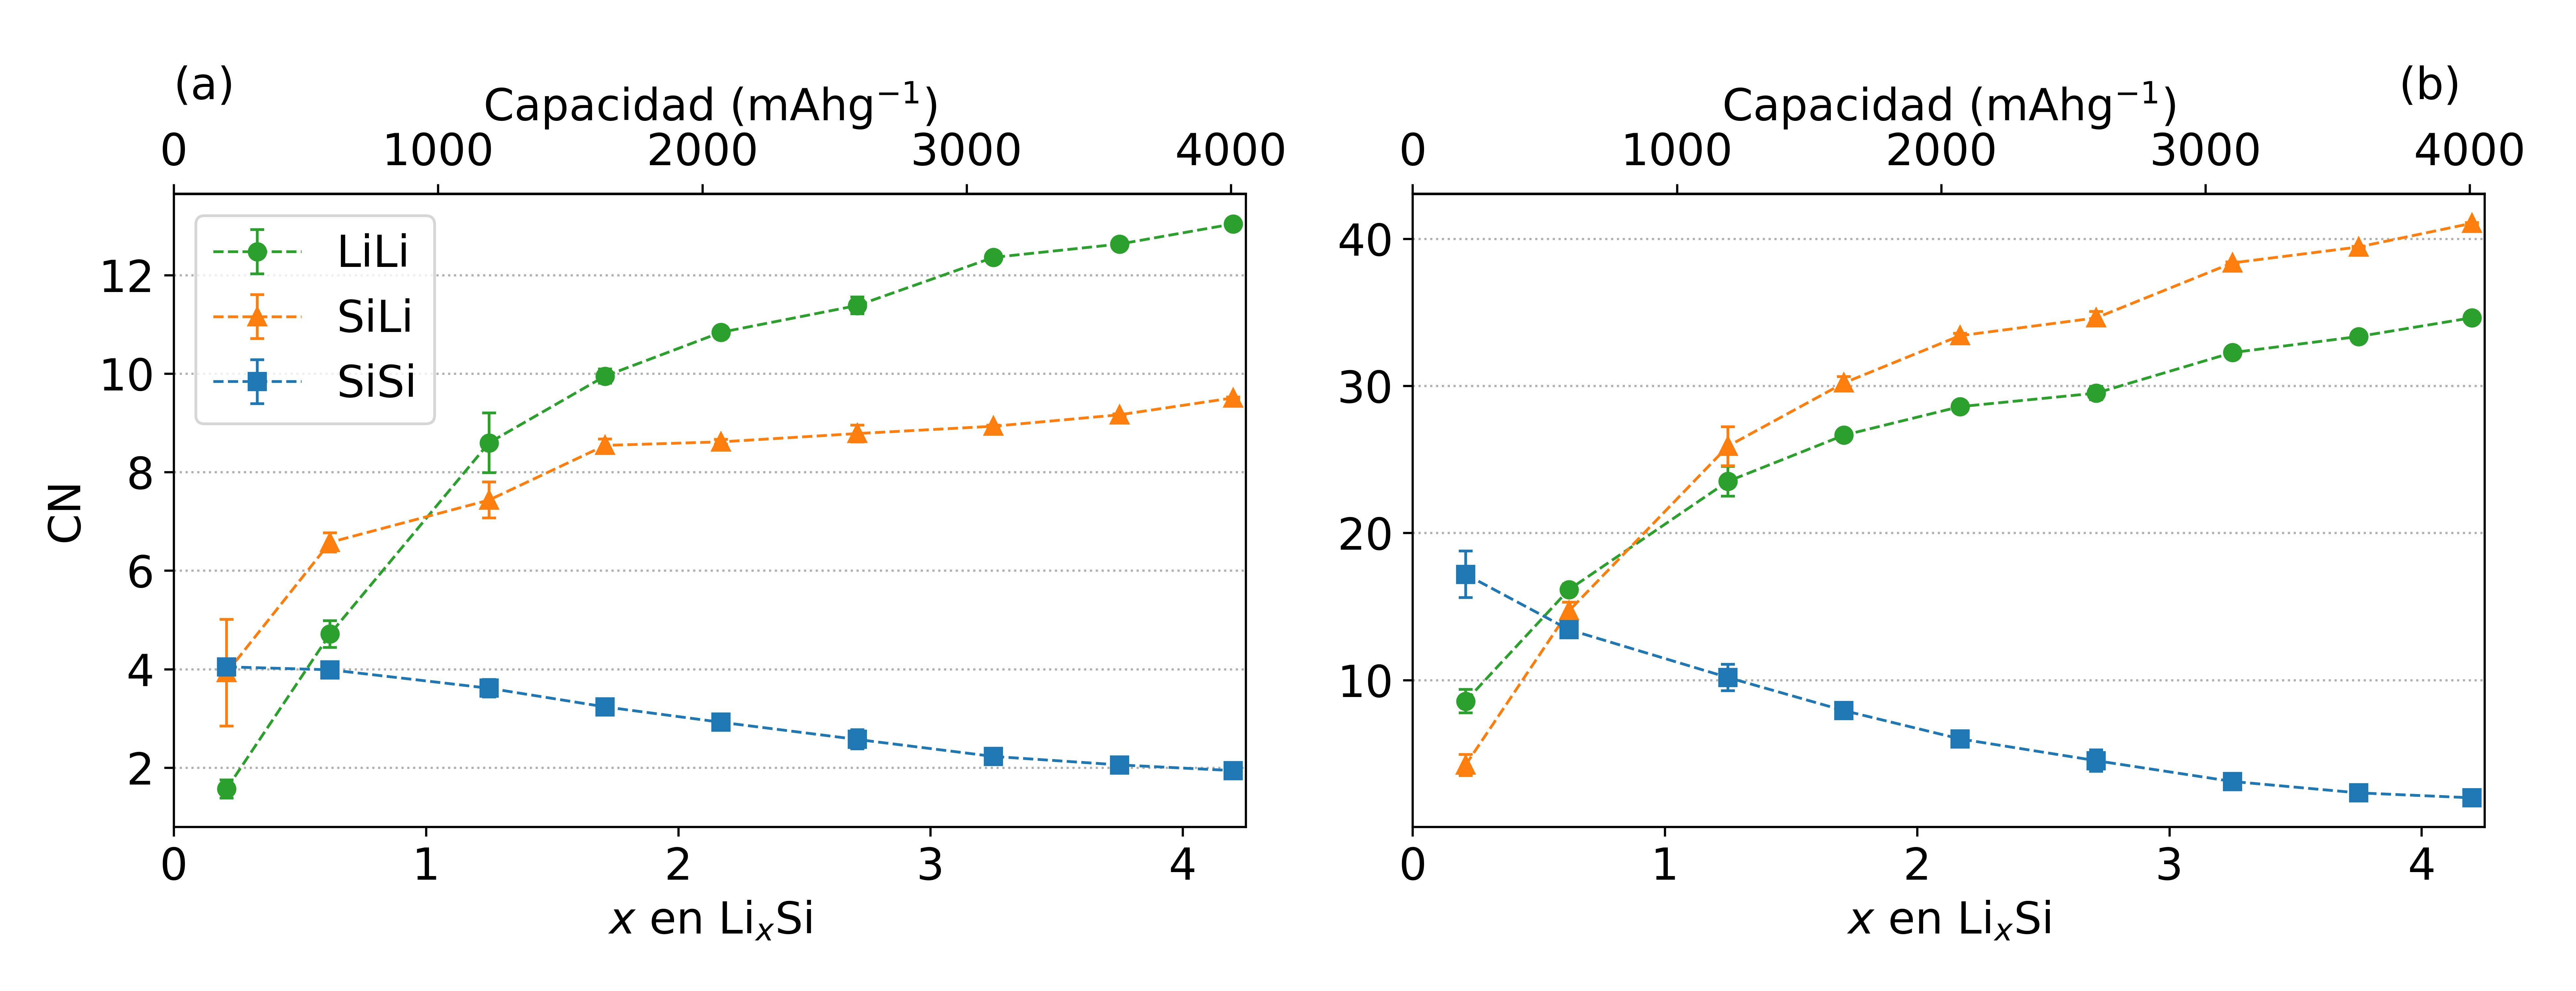
\includegraphics[width=\textwidth]{Silicio/caracterizacion/resultados/cn/cn.png}
    \caption{Número de coordinación en función de la concentración de litio para
    Li-Li, Si-Si y Si-Li. Como radios de corte se utilizaron las distancias 
    del pico de la RDF correspondiente. En los casos en que no se aprecia la barra
    de error, la misma es menor que el tamaño de los puntos. (a) Primero número 
    de coordinación. (b) Segundo número de coordinación.}
    \label{fig:cn}
\end{figure}

Para el caso del CN$_{\text{Si}-\text{Si}}$, se tiene que esta cantidad decrece de 4 a 2, a 
medida que la concentración de Li aumenta. Esto indica que a valores pequeños de 
$x$ la estructura de Si mantiene sus conexiones tetraédricas, mientras que para
valores grandes de $x$ el Si tiende a formar cadenas periódicas unidimensionales.
En la red de silicio amorfa, analizada con más detalle en la sección 
\ref{s:clusters}, se presenta una estructura 3d-periódica para valores bajos de 
$x$, donde el CN se encuentra alrededor de 4. Luego, se alcanza una estructura 1d-periódica 
para valores grandes de $x$, donde los enlaces Si-Si tienden a formar 
cadenas, que pueden verse para $x = 3.75$ donde se tiene CN = 2.05, por ejemplo.
El CN de Si-Li y Li-Li presenta valores pequeños para concentraciones 
bajas y aumenta monótonamente hasta alcanzar valores de 10 y 12, respectivamente, 
que se asemejan al valor de una estructura de empaquetamiento compacto.

Los resultados para el segundo número de coordinación se presentan en la Figura 
\ref{fig:cn}b. Estos resultados se obtuvieron considerando un cascarón con un 
radio de corte interno y otro externo, elegidos de manera tal que incluyan el 
segundo pico de la RDF. La elección de dichos valores varió dependiendo del tipo
de átomos que se consideraron. En todos ellos se tomó como radio de corte interno 
el radio de corte del primero número de coordinación. Luego, para el radio de 
corte externo se utilizaron valores de 5.0 \AA\ para Si-Si y 6.0 \AA\ para Li-Li
y Si-Li.

Para los valores de CN$_{\text{Si}-\text{Si}}$ se observa un aumento para concentraciones bajas
de Li, si se lo compara con el CN de primeros vecinos. Para valores mayores de $x$,
se puede ver cómo el valor de CN también tiende a 2, lo cual es coherente con la
formación de cadenas que se notó previamente. La tendencia cualitativa del segundo
CN para Li-Li y Si-Li es la misma que la observada en el primer CN, sólo que ahora
empieza en un valor cercano a 5 y tiende a 35 y 40, respectivamente. Este valor 
es mucho mayor que el que se tiene para los segundos vecinos en una estructura 
de empaquetamiento compacto, que es 6 para la estructura cristalina FCC. Incluso 
es mayor a la suma del segundo (6) y del tercer vecino (24) esperado para la red 
FCC.


% Copyright (c) 2024, Francisco Fernandez
% License: CC BY-SA 4.0
%   https://github.com/fernandezfran/thesis/blob/main/LICENSE
\subsection{Formación de conglomerados (clusters)}\label{s:clusters}

Analizando la formación de \change{conglomerados} (clusters) por medio del algoritmo DBSCAN 
\cite{ester1996}, en el cual puede definirse un radio de corte para el cual se 
deja de considerar que los átomos están enlazados entre sí (es decir, formando 
clusters), se encuentra que las estructuras amorfas de silicio no pueden ser 
clasificadas en diferentes tipos de clusters, las mismas reflejan más bien 
una red amorfa. Esto viene de interpretar los gráficos que se presentan en la 
Figura \ref{fig:clusters}. 
\begin{figure}[h!]
    \centering
    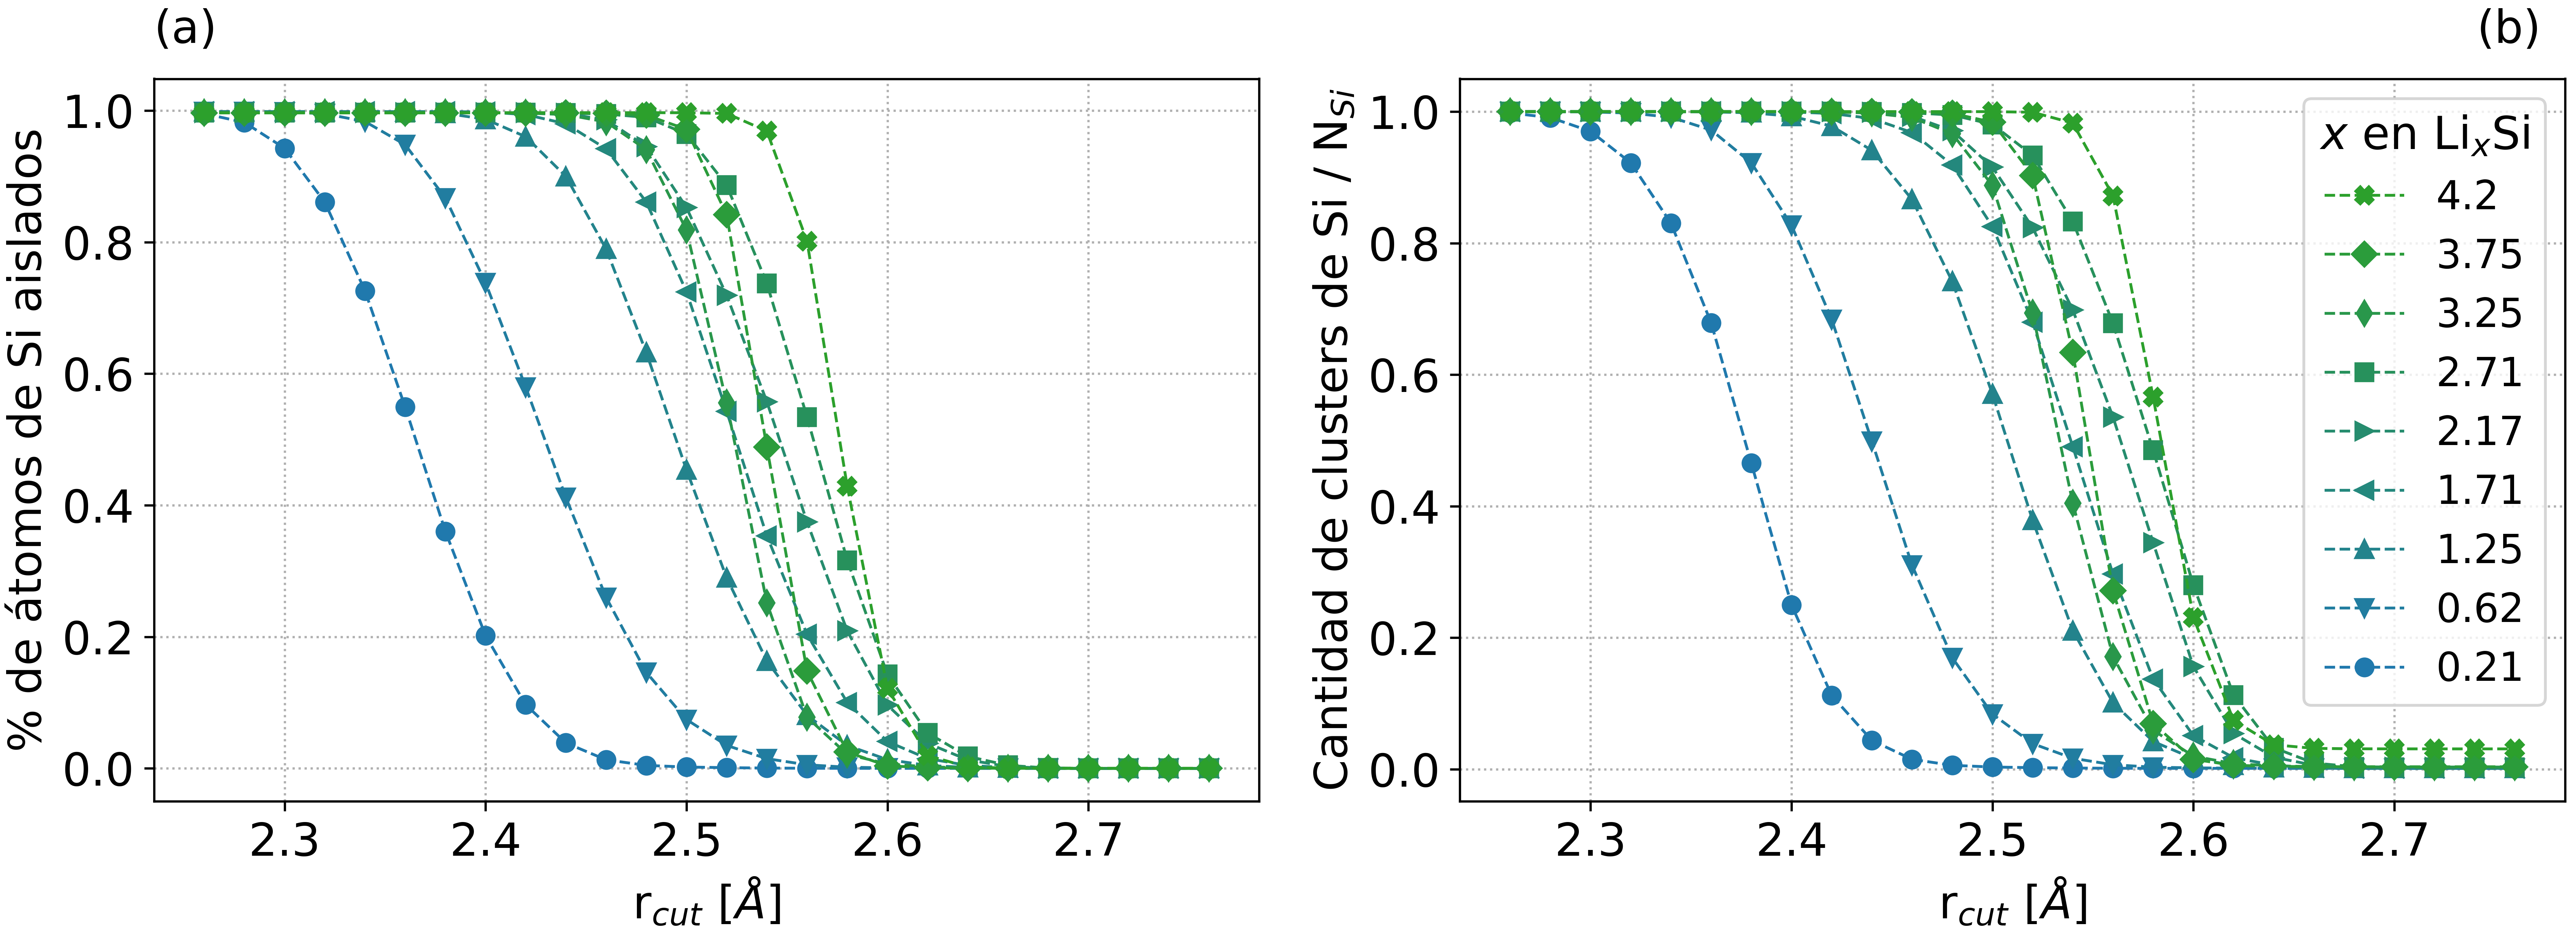
\includegraphics[width=\textwidth]{Silicio/caracterizacion/resultados/clusters/clusters.png}
    \caption{Formación de clusters indicando una red amorfa de silicio. (a) 
    Fracción de átomos de Si aislados en función de la elección del
    radio de corte. (b) Número de clusters de Si sobre el número total de átomos 
    de Si.}
    \label{fig:clusters}
\end{figure}

En particular, en la Figura \ref{fig:clusters}a se define la fracción 
de átomos de Si que están a una distancia mayor que $r_{cut}$ de otros átomos de 
Si. Cuando el radio de corte es mayor que la distancia a la cual termina el 
primer pico de la RDF$_{\text{Si}-\text{Si}}$, no se tienen átomos de Si que cumplan esta 
propiedad, es decir, no hay átomos de Si que se encuentren aislados en el sistema,
incluso a concentraciones altas de Li. Esto refleja que el a-Si se comporta como 
una red en la cual todos los átomos de silicio están interconectados entre sí, 
cosa que también se puede deducir de la Figura \ref{fig:clusters}b, en la cual 
se tiene que cuando el radio de corte es menor que el primer pico de la RDF$_{\text{Si}-\text{Si}}$ 
el número de clusters es igual al número de átomos de Si, pero que cuando este 
radio es más grande que la distancia a la cual termina el primer pico, hay un 
solo cluster.


\subsection{Interconexión de clusters}\label{s:interconexion}

Para determinar qué es lo que genera una estructura compleja en el segundo pico de la 
RDF$_{\text{Si}-\text{Li}}$, ver Figura \ref{fig:rdf}, se realizó un análisis similar al reportado por Ding \textit{et al.}
\cite{ding2015}. Estos autores analizaron la correlación en la distancia de a
pares de los segundos vecinos más cercanos en términos de las conexiones entre
clusters, definiendo un poliedro de coordinación alrededor del átomo central 
considerado para la RDF y sus segundos vecinos. El número de átomos compartidos
entre estos dos poliedros de coordinación enlazados fueron utilizados para 
establecer categorías y analizar sus contribuciones a la RDF. Estas categorías
dependen del hecho de que los poliedros comparten un vértice (1 átomo), una 
arista (2 átomos), una cara de los poliedros (3 átomos) o cuadriláteros 
distorsionados o tetraedros aplastados (4 átomos). De una forma similar al trabajo de Ding, se deconvolucionó el segundo pico de la RDF calculando la RDF parcial 
de distintas categorías, donde cada categoría se define por el número de átomos de
Li que interconectan un átomo de Si con su segundo vecino de Li. El comportamiento
detallado se presenta en la Figura \ref{fig:interconexiones}. Puede afirmarse a 
grandes rasgos que para concentraciones bajas de Li en las aleaciones, hay una 
predominancia de segundos vecinos de Li que tienen una o ninguna interconexión 
con los vecinos de Li de la primera esfera de coordinación Si-Li. Para $x > 1.0$
la contribución del segundo vecino de Li interconectado con dos o más átomos de 
Li de la primera esfera de coordinación Si-Li comienza a ser predominante y la
contribución de los átomos de Li sin conectarse empieza a decaer. Para $x > 3.0$,
la contribución del primer pico del segundo vecino de Li interconectado dos o
tres veces se vuelve relevante mientras que aparecen contribuciones de cuatro o
más interconexiones.
\begin{figure}[h!]
    \centering
    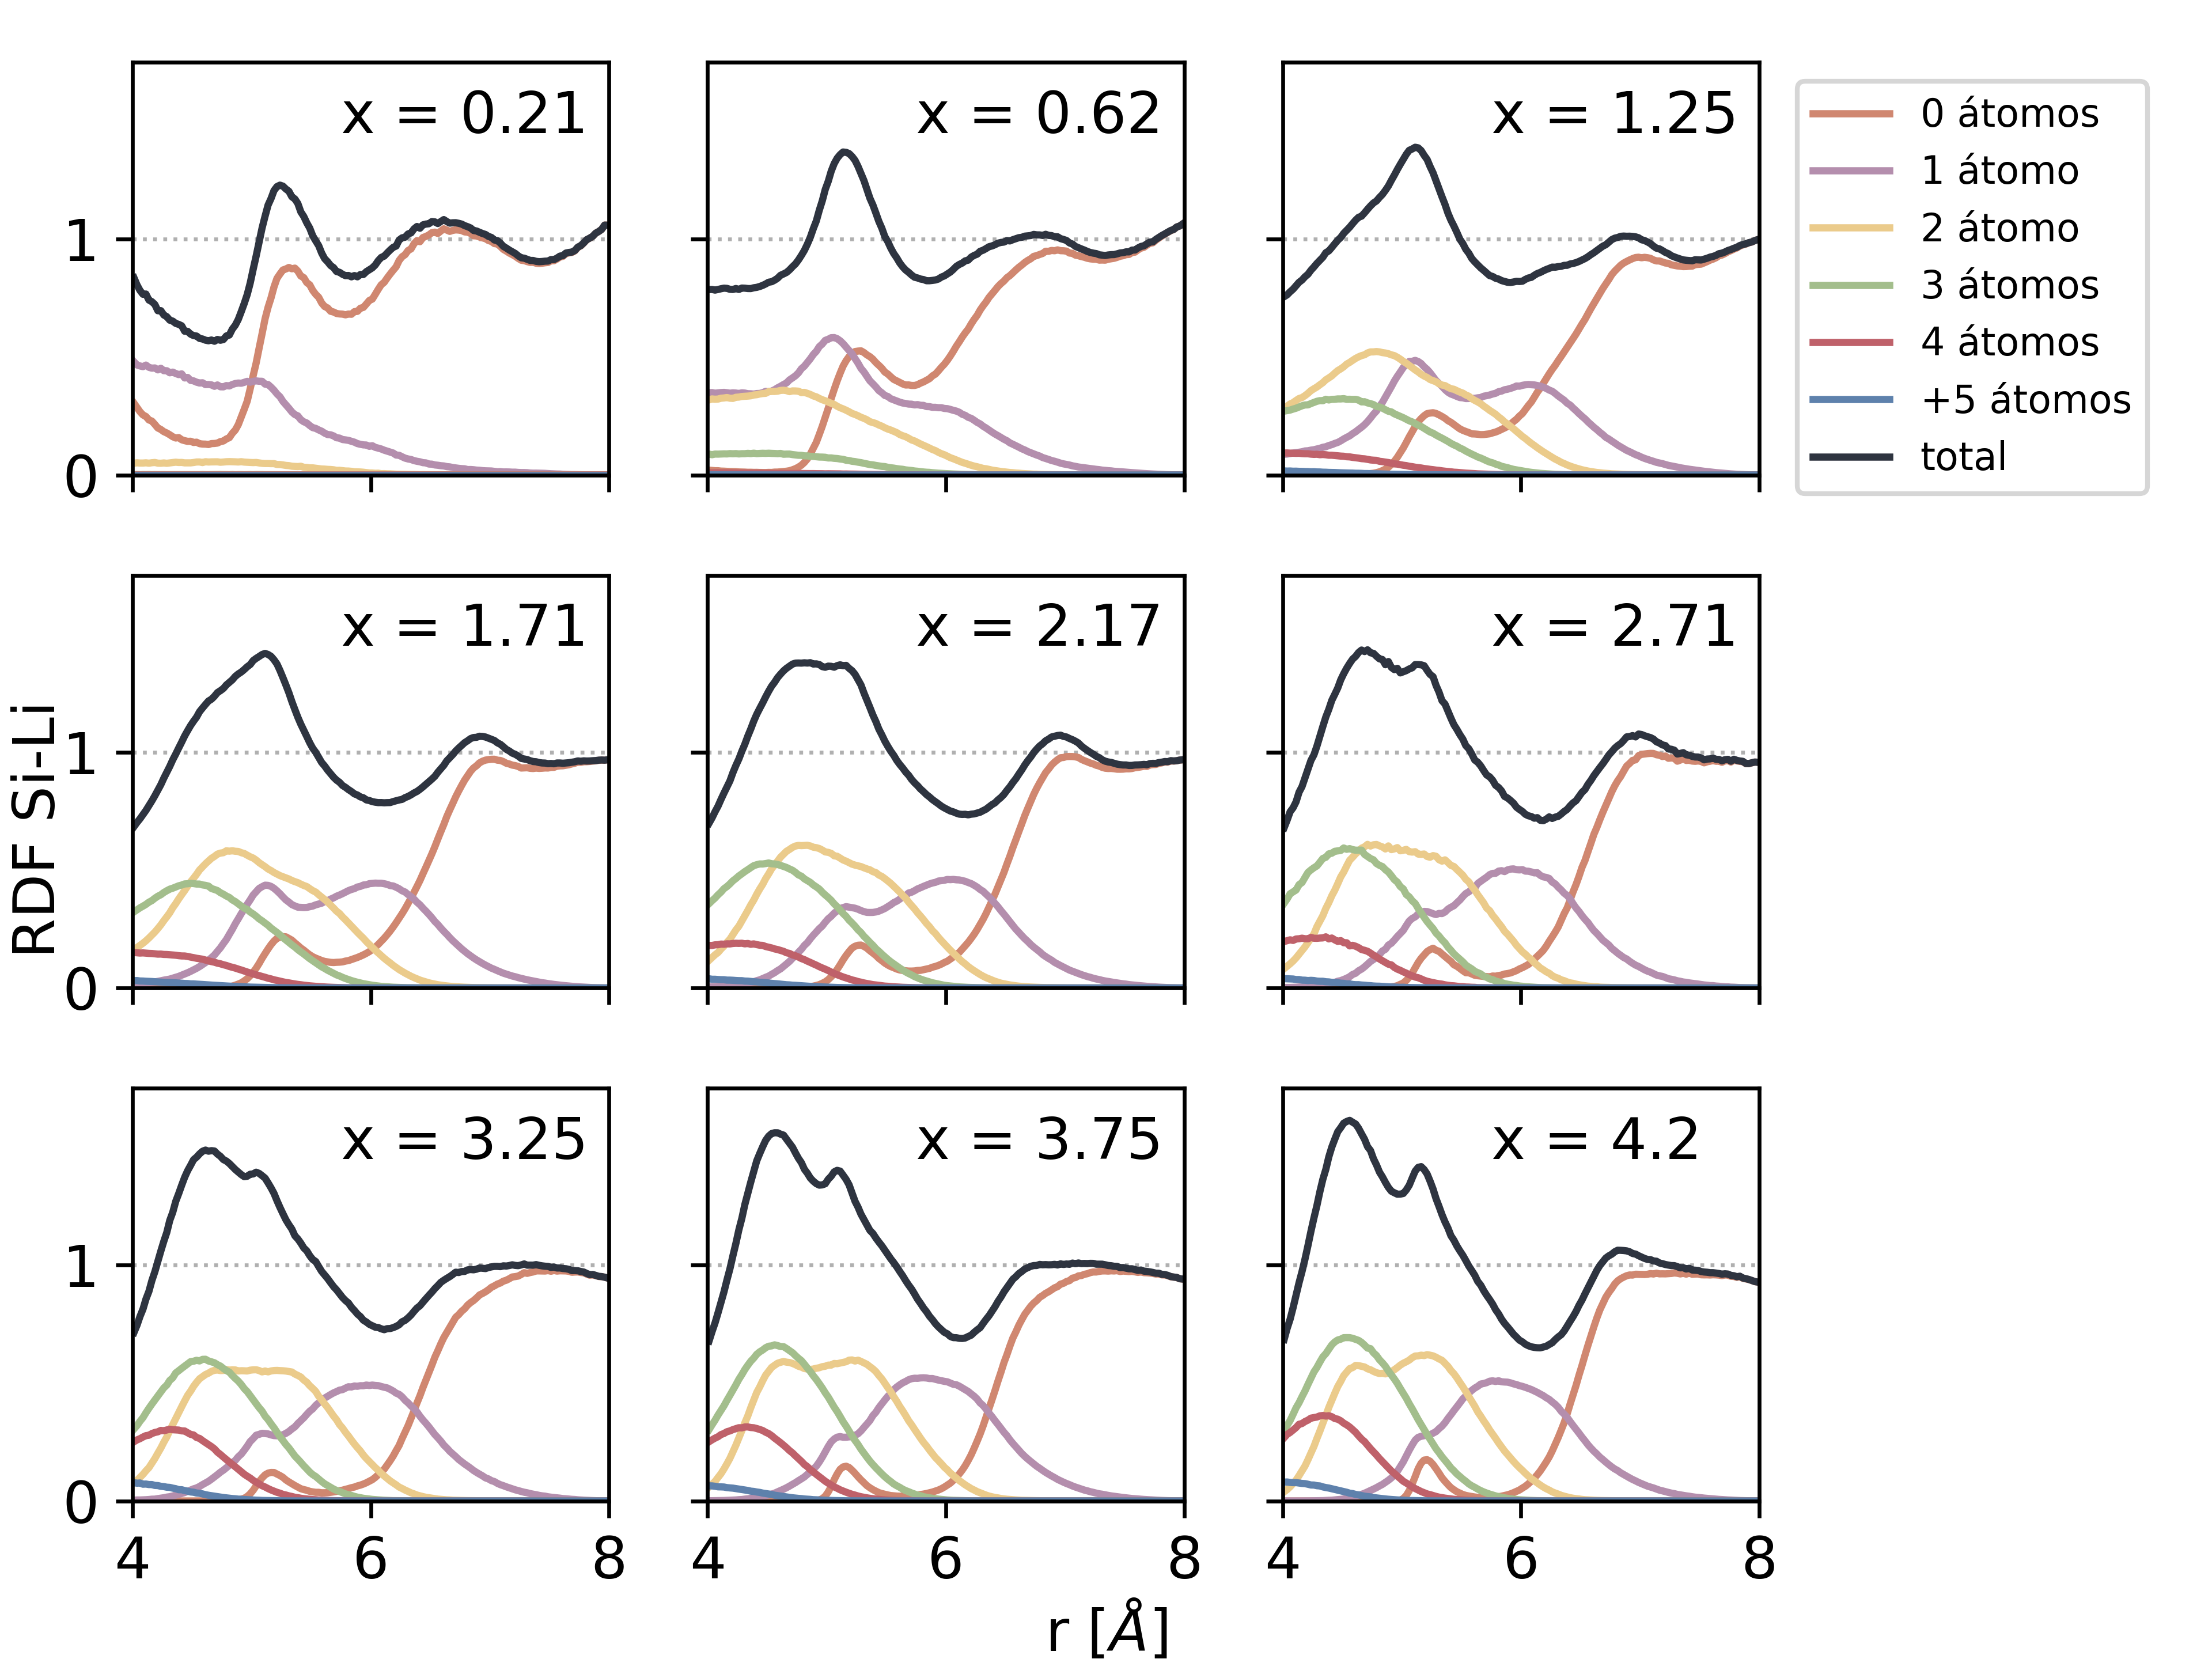
\includegraphics[width=\textwidth]{Silicio/caracterizacion/resultados/interconexion/interconexiones.png}
    \caption{Interconexiones de los segundos vecinos más cercanos de Li con un 
    átomo central de Si para cada valor de $x$ en Li$_x$Si considerado \cite{ding2015}. El número 
    de primeros vecinos más cercanos que conectan a los segundos vecinos más 
    cercanos con el átomo central de Si se indica en el recuadro de las figuras. 
    Además de la RDF$_{\text{Si}-\text{Li}}$ total, se grafica cada una de las contribuciones 
    de los diferentes tipos de interconexiones posibles.}
    \label{fig:interconexiones}
\end{figure}

Mientras que el comportamiento presentado en la Figura \ref{fig:interconexiones}
es más bien complejo, pueden establecerse tendencias generales que ayudan a 
entender mejor que es lo que sucede. Si se divide la RDF$_{\text{Si}-\text{Li}}$ en dos 
contribuciones de segundos vecinos, la primera de ellas, que se encuentra a una
distancia entre 4.0 \AA\ y 5.0 \AA, se puede atribuir a los átomos que tienen dos 
o más interconexiones de Li, mientras que la segunda de ellas, entre 5.0 \AA\ y
5.6 \AA, se corresponde con los átomos que tiene una o ninguna interconexión de 
Li. Utilizando esta clasificación, se muestra en la Figura 
\ref{fig:interconexiones-areas} la fracción del área que representa cada una de
estas categorías en función de la concentración de litio.
\begin{figure}[h!]
    \centering
    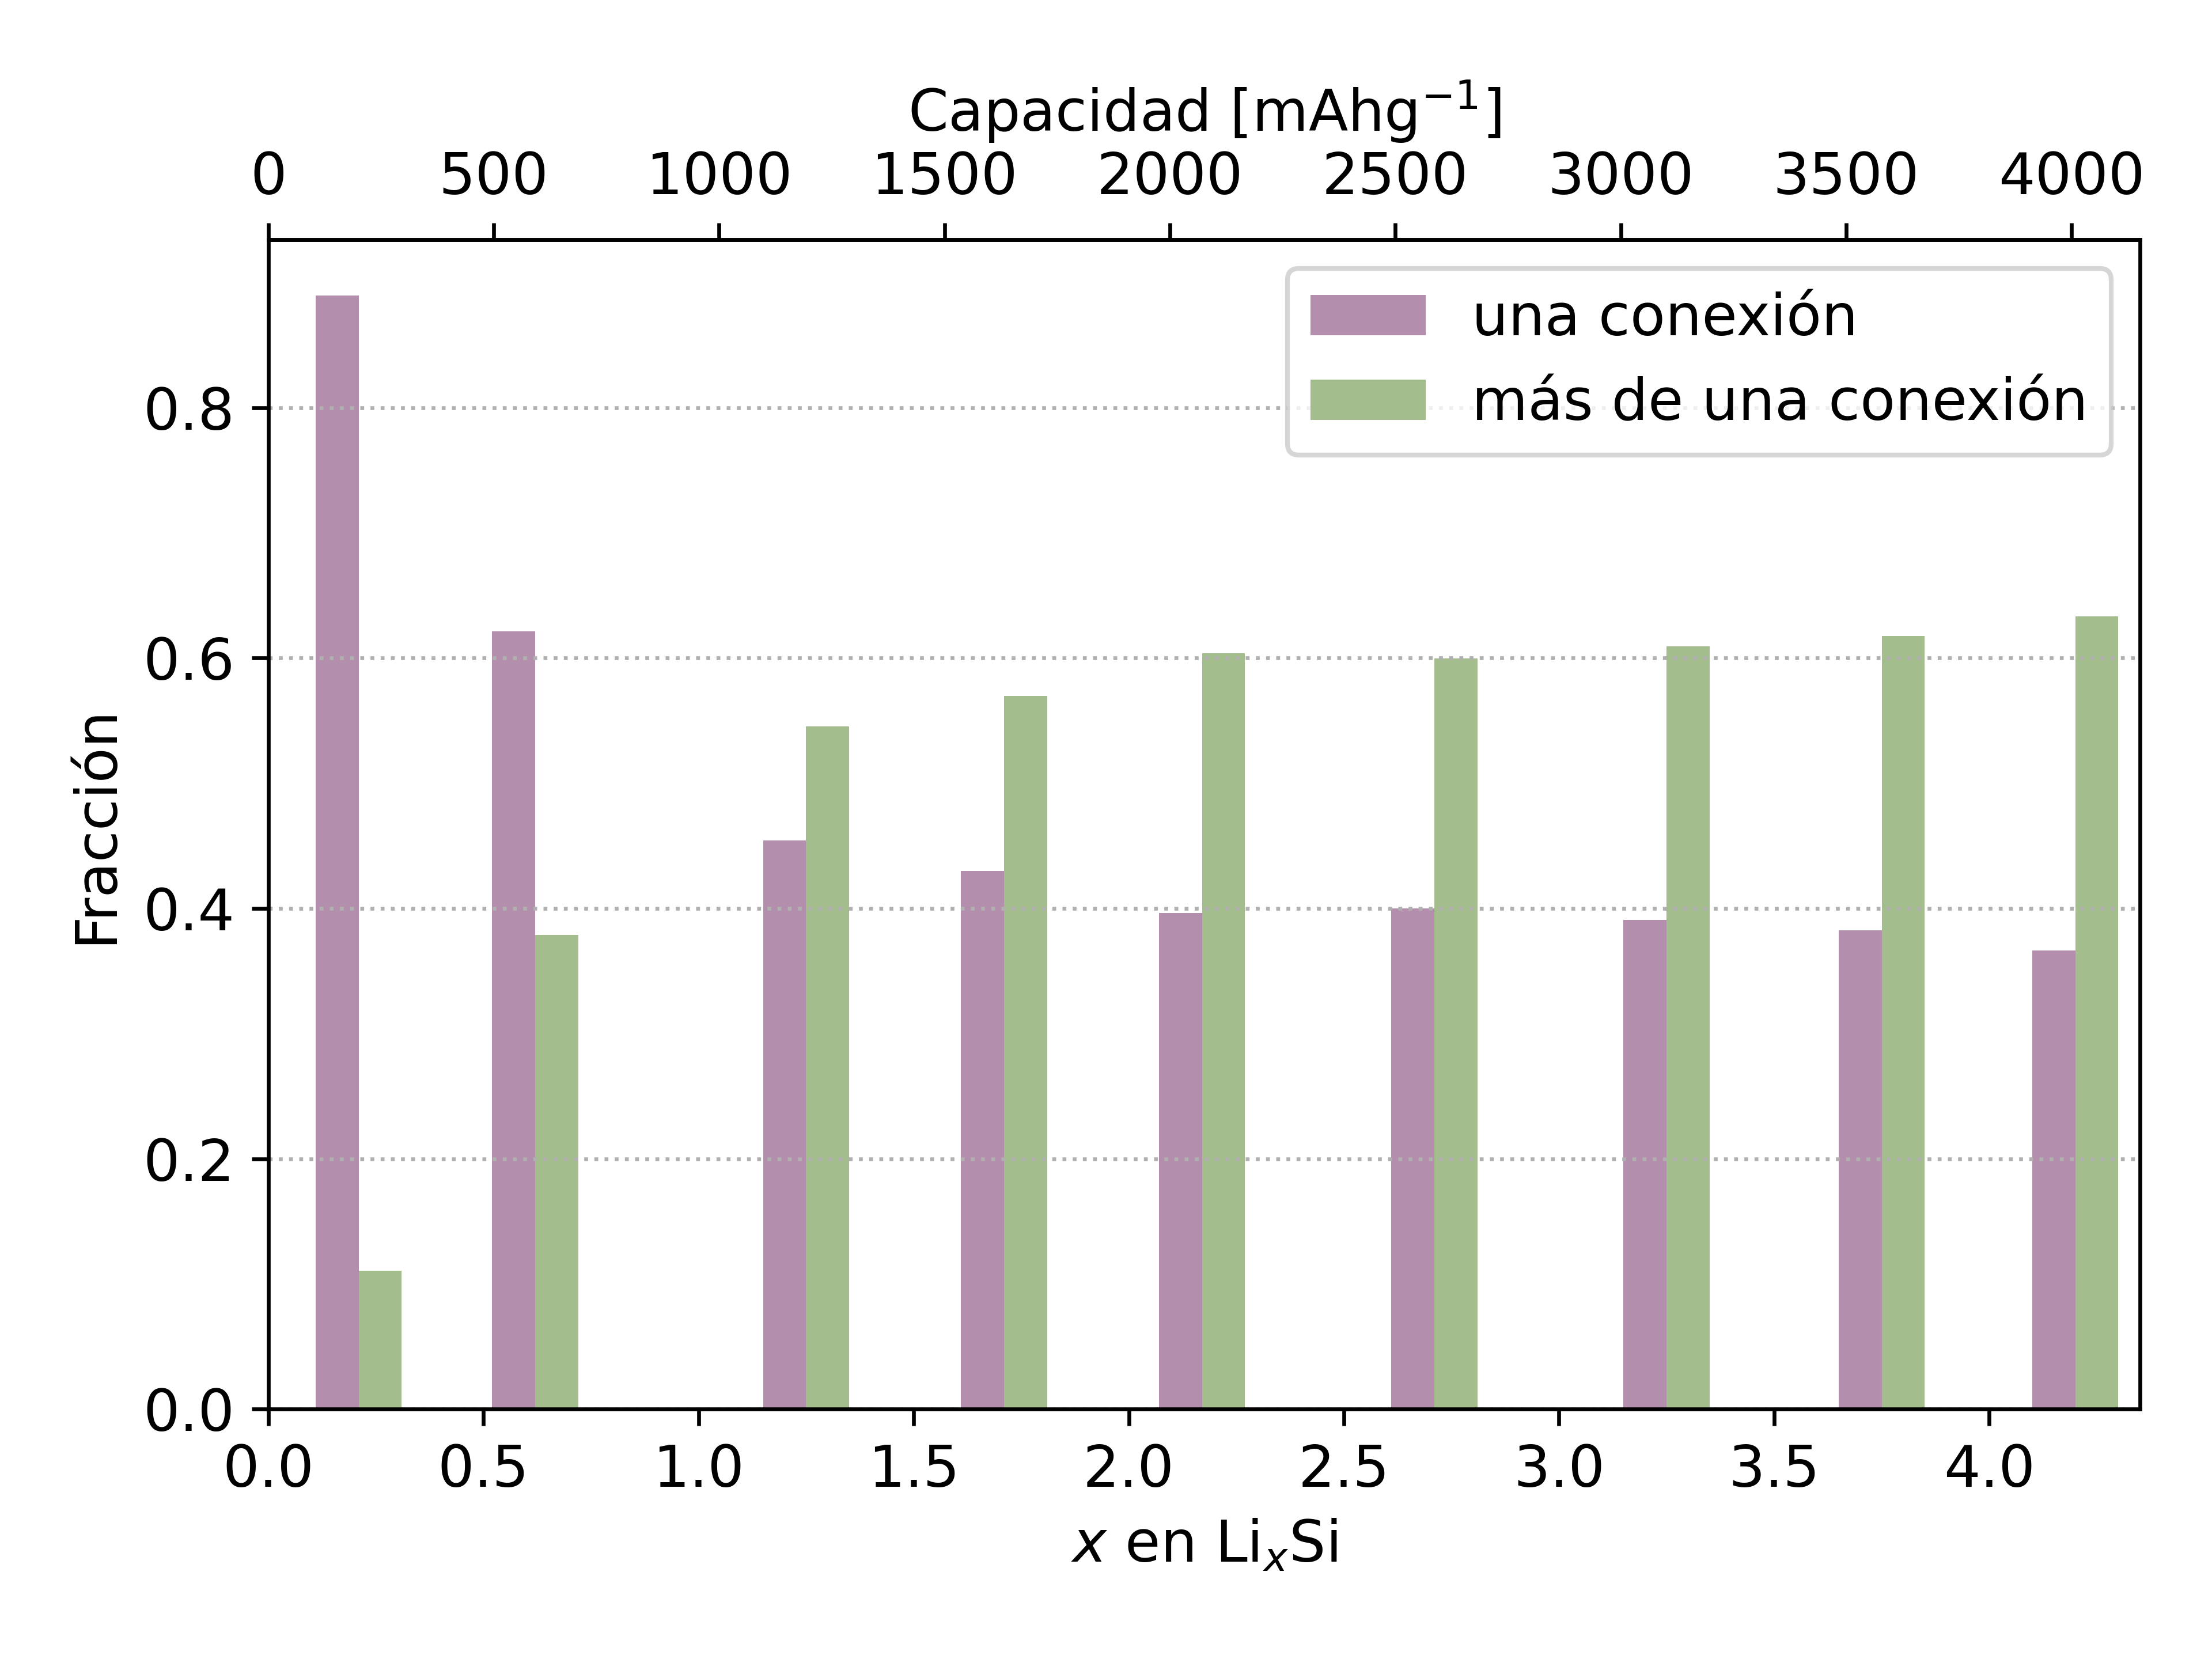
\includegraphics[width=0.7\textwidth]{Silicio/caracterizacion/resultados/interconexion/interconexiones-areas.png}
    \caption{Evolución con la concentración de la fracción que representa cada
    categoría de interconexiones de Li al área total del segundo pico de la 
    RDF$_{Si-Li}$.}
    \label{fig:interconexiones-areas}
\end{figure}


\subsection{Orden de corto alcance}

El término orden de corto alcance (SRO, de sus siglas en inglés 
\textit{short-range order}) se utiliza para denotar el ordenamiento de los átomos
que rodean a uno específico en una cáscara. Del mismo modo, el término 
\textit{clustering} se ha definido como la tendencia de los átomos similares a 
estar cerca unos de otros. Ambos conceptos se refieren a un orden estructural 
entre átomos vecinos, pero no son necesariamente persistentes a distancias más 
largas. Warren ~\cite{warren69} y Cowley ~\cite{cowley1950} definieron un 
parámetro (WCP) para caracterizar estos tipos de ordenamientos de la siguiente 
manera:
\begin{equation}
    WCP = 1 - \frac{p_{A-B}}{m_B} = 1 - \frac{p_{B-A}}{m_A},
\end{equation}
donde $p_{A-B}(p_{B-A})$ es la probabilidad de tener un átomo de tipo B(A) como
vecino de un átomo de tipo A(B) y $m_B(m_A)$ es la concentración global de átomos
B(A), expresadas en fracciones molares. La igualdad, en ambas definiciones 
posibles del WCP, viene del hecho de que la probabilidad de encontrar a un átomo 
de tipo A como vecino de un átomo de tipo B es igual a la de tener un átomo de 
tipo B como vecino de un átomo de tipo A, esto es $m_A p_{A-B} = m_B p_{B-A}$.

Los valores que se obtienen de utilizar el parámetro WCP en sistemas del tipo
A$_x$B indica una aleatoriedad completa si es igual a cero, preferencia por 
átomos de distinto tipo si $WCP < 0$ y preferencia por átomos del mismo tipo si 
$WCP > 0$. Aunque este parámetro permite un análisis cuantitativo notable, sólo
se define para sistemas cristalinos en los que cada átomo tiene el mismo número
de vecinos. ~\cite{warren69}

A continuación se extiende esta idea para definir un nuevo parámetro, 
$\theta_{A-B}$, que es adecuado para caracterizar estructuras amorfas, de la 
siguiente manera:
\begin{equation}
    \theta_{A-B} = \ln \left( \frac{C_{A-B}}{C_{Bulk}} \right),
\end{equation}
donde A indica la naturaleza del átomo que se considera como central y B el tipo
de átomo que se considera como vecino, equivalente a la definición de WCP. En
este caso, la relación entre la concentración local y la concentración global se 
calcula a partir de la integración de la distribución radial de a pares parcial,
$g_{A-B}(r)$, en una esfera al rededor del átomo central,
\begin{equation}
    \frac{C_{A-B}}{C_{Bulk}} = \frac{1}{V(r_{cut})} \int_0^{r_{cut}} g_{A-B}(r) dV,
\end{equation}
donde $r_{cut}$ y $V(r_{cut})$ son el radio de corte y el volumen de la esfera 
considerada. Ya que en $g_{A-B}(r)$ no hay dependencia angular, $dV$ puede 
escribirse como $4 \pi r^2 dr$. Esta cantidad puede pensarse como la 
concentración promedio dentro de la esfera relativa a la del material 
masivo. Así, de forma análoga al parámetro de WCP, $\theta_{A-B}$ indica 
la tendencia SRO o el \textit{clustering} para cualquier tipo de átomo dado.
Si $\theta$ es positivo, indica una acumulación de átomos relativa al 
\textit{bulk}, mientras que si es negativo indica una disminución. Si es igual a 
cero se tiene una aleatoriedad completa. Este nuevo parámetro también satisface 
la relación $\theta_{A-B} = \theta_{B-A}$ de la misma manera que se discutió para
el parámetro de WCP, ya que por definición $g_{A-B}(r) = g_{B-A}(r)$. Por lo cual 
se tiene que el parámetro $\theta_{A-B}$ da información similar a la que provee 
el WCP, pero además es aplicable a sistemas amorfos.

La figura \ref{fig:sro} muestra la variación del parámetro $\theta$ en función 
de la concentración de Li. Hay tres posibilidades para el análisis de $\theta$ en
sistemas de Li$_x$Si ($\theta_{Li-Li}$, $\theta_{Si-Si}$ y $\theta_{Si-Li}$), ya
que $\theta_{Si-Li} = \theta_{Li-Si}$. Para todos los casos se consideraron los
mismos radios de corte que en los cálculos del número de coordinación, luego del
primer pico de la RDF correspondiente.
\begin{figure}[th]
    \centering
    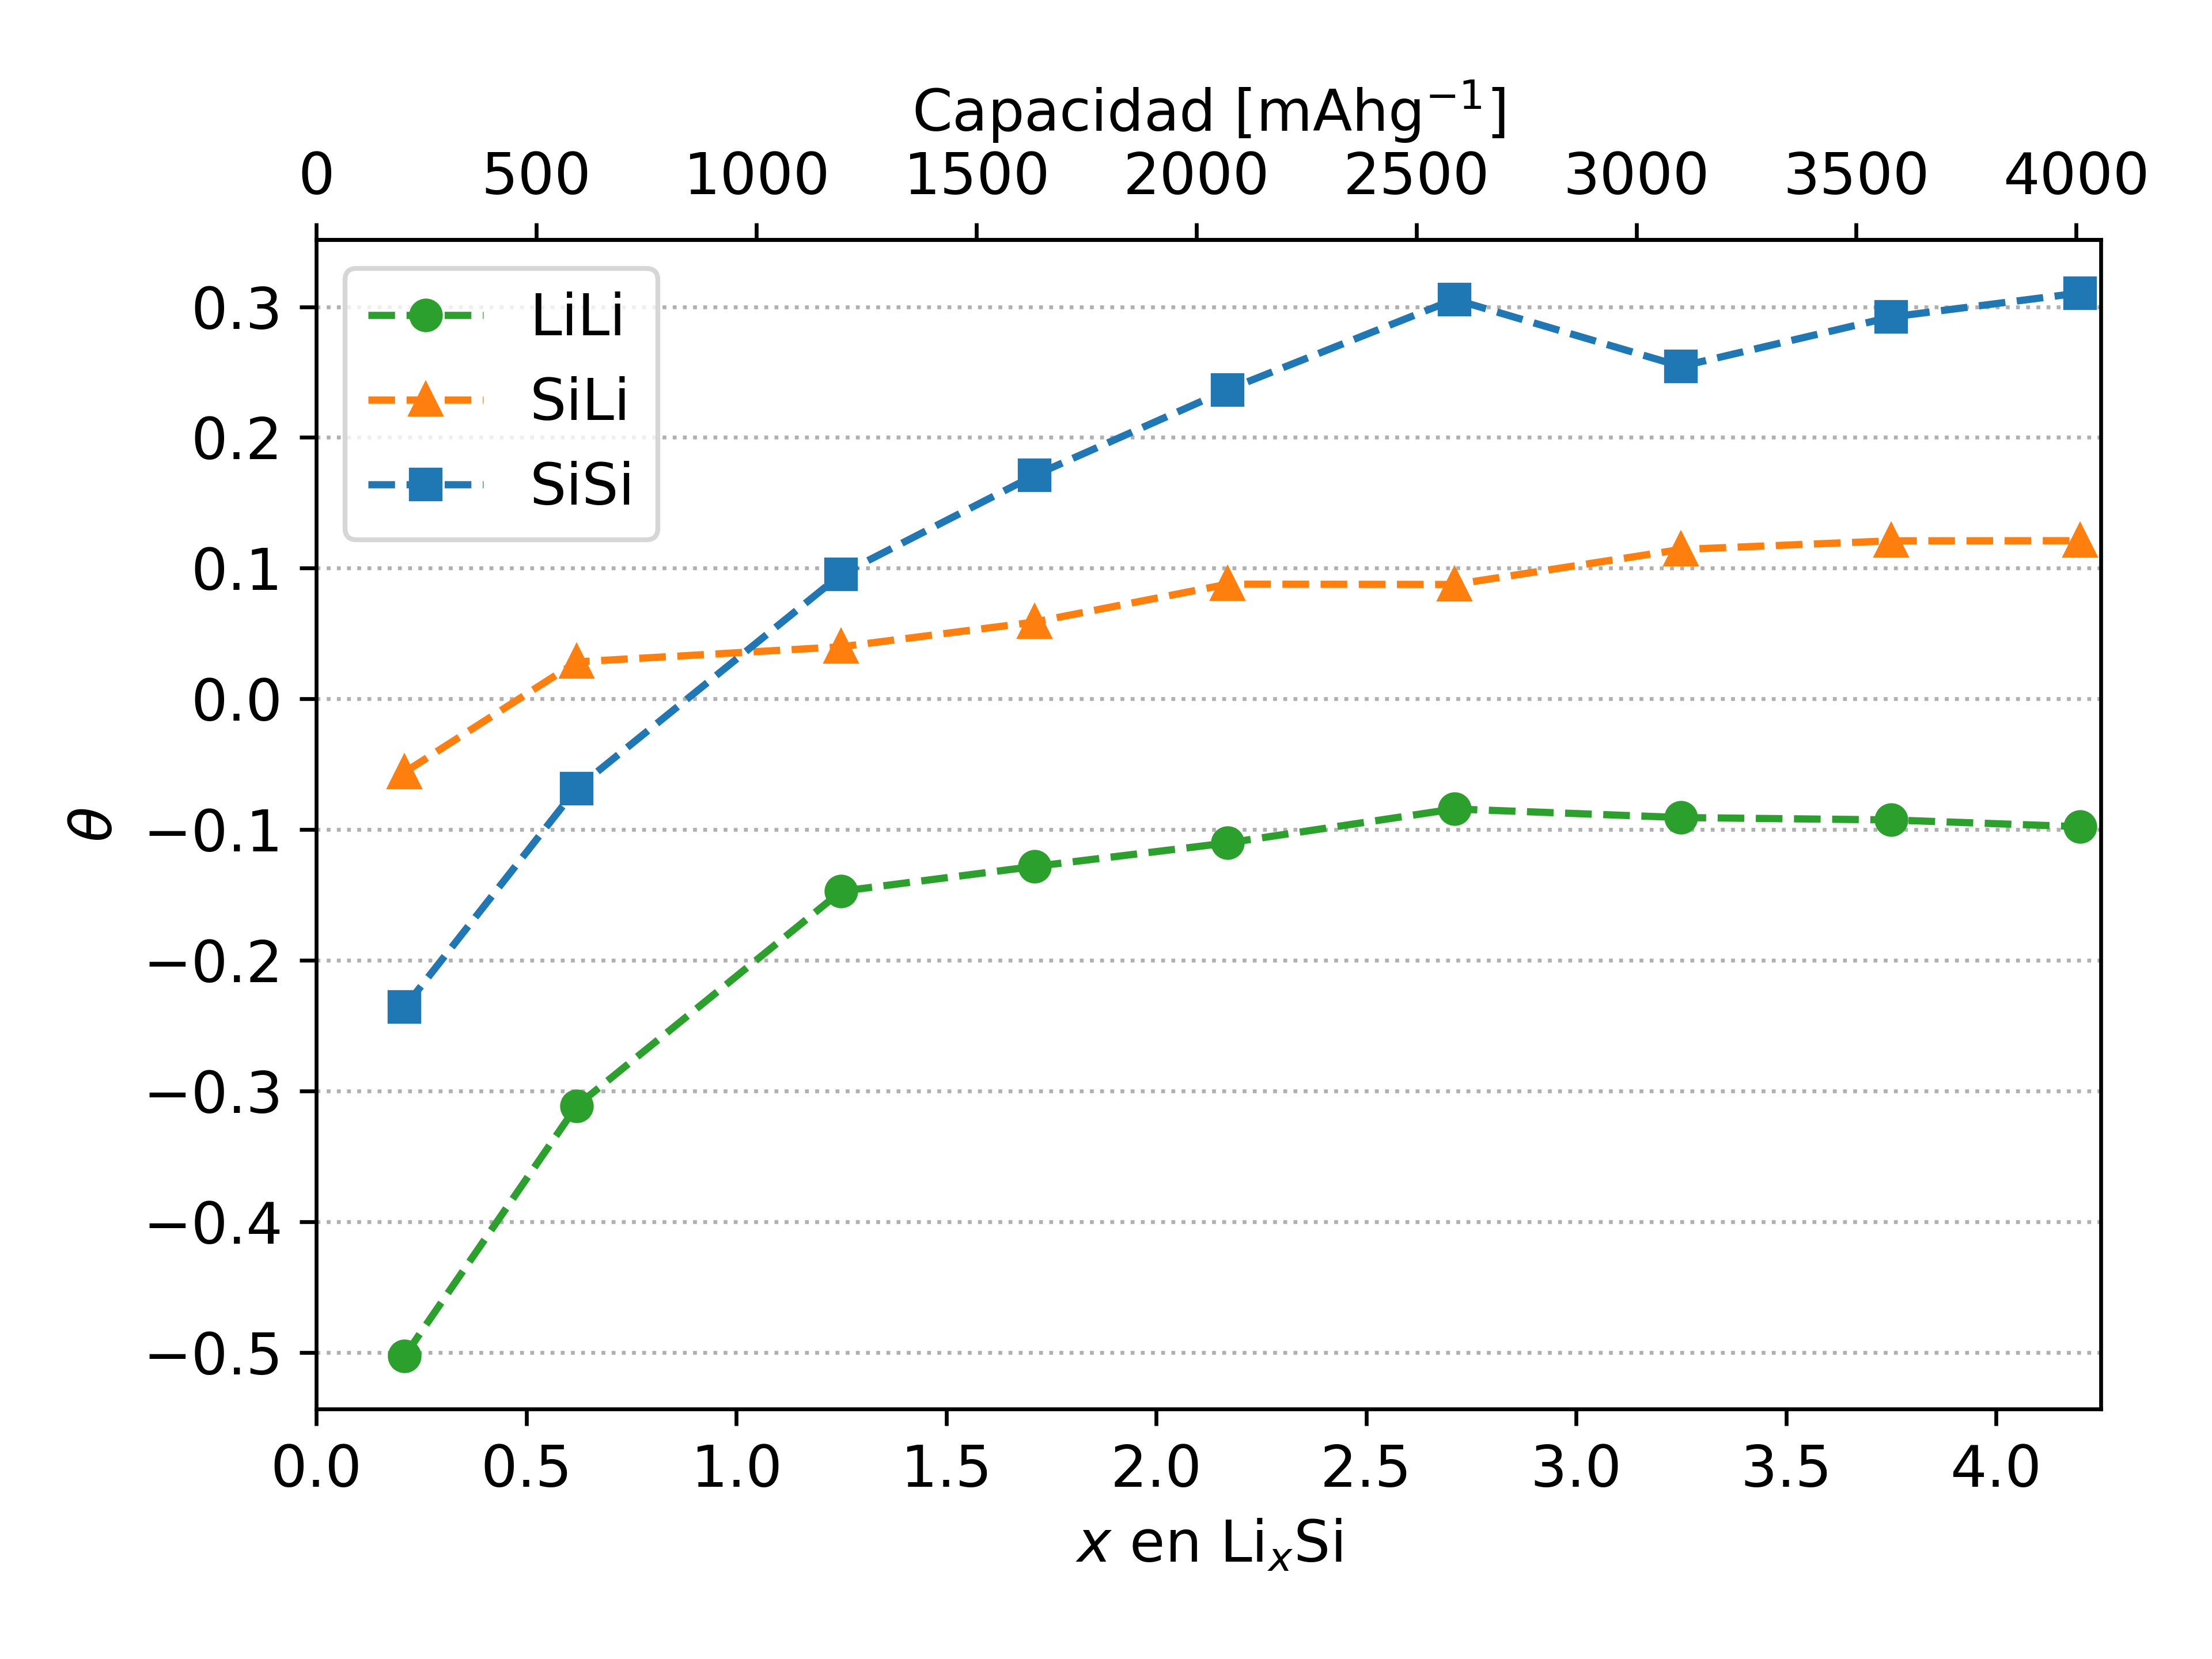
\includegraphics[width=0.8\textwidth]{Silicio/caracterizacion/resultados/sro/sro.png}
    \caption{Parámetros $\theta_{Li-Li}$, $\theta_{Si-Li}$ y $\theta_{Si-Si}$ 
    en función de la concentración de Li. El primer subíndice indica el tipo de
    átomo que se considera como central mientras que el segundo es el vecino. El
    radio de corte se eligió luego del primer pico de la RDF correspondiente.}
    \label{fig:sro}
\end{figure}

Como tendencia general, puede notarse que todos los valores de $\theta$ aumentan
cuando crece la cantidad de litio en el sistema, $x$, y que se estabiliza para 
valores grandes de $x$. Este comportamiento monótono y la disminución en la 
pendiente para concentraciones altas está correlacionado con el comportamiento
presentado en el análisis de los números de coordinación.

En el caso de $\theta_{Si-Si}$, alcanza un valor positivo aproximadamente 
constante para $x > 2.5$, mostrando una correlación fuerte con la presencia de 
cadenas lineales de Si, previamente discutidas y observadas en la figura 
\ref{fig:amorfas}. Aunque la presencia de estas cadenas se puede inferir a partir
de los valores de los CN en $x$ altos, $\theta$ es más sensible al SRO, ya que
está normalizado por la concentración global. Esta propiedad de $\theta$ permite
un análisis más claro incluso si las cadenas están interactuando entre sí, como
es el caso para concentraciones bajas de litio.

$\theta_{Si-Li}$ presenta variaciones pequeñas y un valor positivo para todo 
$x > 0.5$, mostrando una acumulación constante de Li al rededor del Si, o, 
análogamente, una acumulación de Si alrededor del Li. Este comportamiento se le 
puede atribuir a la interacción atractiva fuerte en los pares Si-Li. En el caso de 
$\theta_{Li-Li}$, este parámetro es siempre negativo, lo que indica una 
interacción débil Li-Li y la correspondiente disminución de vecinos Li-Li. Por
último, el parámetro $\theta_{Si-Si}$ tiene un valor negativo para $x < 1.0$, 
sugiriendo que la presencia de concentraciones bajas de litio tiende a separar 
los átomos de silicio entre sí. Sin embargo, $\theta_{Si-Si}$ se vuelve positivo
para $x > 1.0$, implicando una acumulación de vecinos de Si sobre átomos de Si, 
relativo a la concentración global. Esto se debe a la formación de estructuras 
Si-Si. Para $x > 2.5$ puede observarse un valor constante de 
$\theta_{Si-Si} \approx 0.3$, revelando la formación de estructuras estables de 
Si-Si dadas por las cadenas previamente mencionadas.



% Copyright (c) 2024, Francisco Fernandez
% License: CC BY-SA 4.0
%   https://github.com/fernandezfran/thesis/blob/main/LICENSE
\section{Conclusiones del capítulo}

Con el fin de emular las estructuras amorfas encontradas en muchos experimentos 
electroquímicos, en este capítulo se generaron por computadora estructuras desordenadas de 
aleaciones de Li$_x$Si para varios valores de $x$ utilizando un algoritmo de 
dinámica acelerada y un campo de fuerzas reactivo. La exploración acelerada de 
mínimos locales (AELM) permitió la caracterización de una amplia gama de 
estructuras amorfas. El cambio de volumen de las estructuras litiadas en relación 
con el Si está en concordancia con los resultados experimentales de microscopía de fuerza atómica. Las
energías de las estructuras obtenidas representan bien el comportamiento 
electroquímico de la curva de potencial en función de la concentración de Li. Se 
analizó la función de distribución radial de a pares para los diferentes tipos de 
pares atómicos y se dilucidó la estructura compleja del segundo pico del RDF 
Si-Li mediante un análisis de interconexión de clusters. Además, haciendo un 
análisis de la formación de clústeres en función del radio de corte, se demostró 
que las estructuras amorfas no presentan diferentes enlaces de Si ni átomos de Si 
aislados. En su lugar, se encontró que el sistema se comporta como una red amorfa.
Estudiando los números de coordinación de primeros y segundos vecinos para las 
diferentes concentraciones, se mostró que esta red amorfa mantiene las conexiones 
tetraédricas para bajas concentraciones de Li y que tiende a formar cadenas lineales para 
altas concentraciones de Li. Por último, la definición de un nuevo parámetro 
permitió determinar el orden de corto alcance de las estructuras amorfas, definido
por interacciones débiles Li-Li e interacciones fuertes Li-Si y Si-Si. El método propuesto AELM 
resulta ser un método rápido y eficaz para obtener mínimos energéticamente 
relevantes. Se hizo una analogía con el templado simulado múltiple.% Un análisis 
%detallado de la eficiencia de AELM en comparación con otros métodos eficientes 
%como el templado simulado múltiple o los métodos de Monte Carlo es una motivación 
%para trabajos futuros.

